%!TEX TS-program = pdflatex
% prelim.tex -- main prelim file
%
% Wisconsin dissertation template
% Copyright (c) 2008-2009 William C. Benton.  All rights reserved.
%
% This program can redistributed and/or modified under the terms of the LaTeX
% Project Public License Distributed from CTAN archives in directory
% macros/latex/base/lppl.txt; either version 1 of the License, or (at your
% option) any later version.
%
% This program includes other software that is licensed under the terms of the
% LPPL and the Perl Artistic License; see README for details.
%
% You, the user, still hold the copyright to any document you produce with this
% software (like your dissertation).
%

%%% You'll want ``oneside'' for the deposit version, but probably not for any
%%% versions that don't need to meet the UW requirements
%%% MJG - note that the thesis dept updated the pt requirement from 12 to 10
%%% (2013)
\documentclass[10pt,oneside,letterpaper]{memoir}

% preamble.tex -- packages to include
%
% Wisconsin dissertation template
% Copyright (c) 2008 William C. Benton.  All rights reserved.
%
% This program can redistributed and/or modified under the terms
% of the LaTeX Project Public License Distributed from CTAN
% archives in directory macros/latex/base/lppl.txt; either
% version 1 of the License, or (at your option) any later version.
%
% This program includes other software that is licensed under the
% terms of the LPPL and the Perl Artistic License; see README for details.
%
% You, the user, still hold the copyright to any document you produce
% with this software (like your dissertation).

%% Comment out any of these that you don't want
\usepackage{amssymb}
\usepackage{amsmath}
\usepackage{amsthm}
%\usepackage{theorem}
\usepackage{hyperref}

%%%%% LISTINGS package and setup
\IfFileExists{listings.sty}{%
\usepackage{listings}%
}{}

%% Packages added by Matt Gidden
%%
%% Note, order matters!
%%
\usepackage{cite} % right order for multiple entries in cite
\usepackage{moreverb} % for verbatim snippets of code
\usepackage{fancyvrb}
\usepackage{tabularx} % for tables with line breaks
\usepackage{threeparttable} % for tables with notes
\usepackage[capitalize, noabbrev]{cleveref} % for reference multiple figures
\usepackage{calc} % allows for arithmetic on latex variables
\usepackage{float} % allows for figures to be placed explicitly
\usepackage{algorithm2e} % for algorithms
\usepackage{subfig}
\usepackage{multirow} % combining rows in tables
\usepackage{footnote}
\usepackage{titlesec} % for using \titleformat
\usepackage{slashbox} % for tables with a divided cell, see http://tex.stackexchange.com/questions/7262/diagonally-divided-table-cell
\usepackage{bashful}
\usepackage{xspace}
\usepackage{color}
\definecolor{listinggray}{gray}{0.9}
\definecolor{lbcolor}{rgb}{0.9,0.9,0.9}
\lstset{
    %backgroundcolor=\color{lbcolor},
    language={C++},
    tabsize=4,
    rulecolor=\color{black},
    upquote=true,
    aboveskip={1.5\baselineskip},
    belowskip={1.5\baselineskip},
    columns=fixed,
    extendedchars=true,
    breaklines=true,
    prebreak=\raisebox{0ex}[0ex][0ex]{\ensuremath{\hookleftarrow}},
    frame=single,
    showtabs=false,
    showspaces=false,
    showstringspaces=false,
    basicstyle=\scriptsize\ttfamily\color{black},
    keywordstyle=\color[rgb]{0,0,1.0},
    commentstyle=\color[rgb]{0.133,0.545,0.133},
    stringstyle=\color[rgb]{0.627,0.126,0.941},
    numberstyle=\color[rgb]{0,1,0},
    identifierstyle=\color{black},
    captionpos=t,
}
\lstdefinestyle{BashOutputStyle}{
  basicstyle=\small\ttfamily,
  numbers=none,
  frame=tblr,
  columns=fullflexible,
  backgroundcolor=\color{blue!10},
  linewidth=0.9\linewidth,
  xleftmargin=0.1\linewidth
}
%
% Adding for some table features
\usepackage{array}
%
% Adding package for float barriers
\usepackage{placeins}

%% Custom commands added by Matt Gidden
\setcounter{tocdepth}{2}
\setcounter{secnumdepth}{3}
\theoremstyle{plain}
\newcommand{\Cyclopts}{\textsc{Cyclopts} }
\newcommand{\Cycamore}{\textsc{Cycamore} }
\newcommand{\cyclus}{\textsc{Cyclus}\xspace}
\newcommand{\Cyclus}{\textsc{Cyclus} }
\newcommand{\nucl}[2]{
\ensuremath{^{#1}}\mbox{#2}
}
\newcommand{\horizfig}[2][]{%
  \begin{minipage}{3in}\subfloat[#1]{#2}\end{minipage}}
%% \newcommand{\code}[1]{\lstinline[basicstyle=\ttfamily\color{green!40!black}]|#1|}
\newcommand{\code}[1]{\lstinline[basicstyle=\ttfamily\color{black}]|#1|}
\newcommand{\codeb}[1]{\texttt{#1}}
\newcommand{\units}[1] {\:\text{#1}}%
\newcommand{\citeme}{\textcolor{red}{CITE}\xspace}
\newcommand{\TODO}[1] {{\color{red}\textbf{TODO: #1}}}%
\newcommand{\Reactor}[1]{\texttt{Reactor{#1}}}
\newcommand{\UOXSource}{\texttt{UOX\_Source}}
\newcommand{\MOXSource}{\texttt{MOX\_Source}}
\newcommand{\Enrichment}{\texttt{Enrichment}}
\newcommand{\ffc}{$f_{\text{fc}}$\xspace}
\newcommand{\frx}{$f_{\text{rx}}$\xspace}
\newcommand{\floc}{$f_{\text{loc}}$\xspace}
\newcommand{\dloc}{$\delta_{\text{loc}}$\xspace}
\newcommand{\dreg}{$\delta_{\text{reg}}$\xspace}
\newcommand{\cbc}{Cbc\xspace}
\newcommand{\clp}{Clp\xspace}

%% You should use natbib
\IfFileExists{natbib.sty}{%
  \usepackage[numbers]{natbib}% added the numbers option from the original WI
                              % thesis template
}{}

%% You probably need appendix, if you want appendices
\IfFileExists{appendix.sty}{%
\usepackage{appendix}%
}{}

%% the spacing in memoir is weird, you'll need to use this
\DisemulatePackage{setspace}
\usepackage[onehalfspacing]{setspace}

%% List setup; the ``hanglist`` environment will allow you to have
%% nicely-typeset enumerated lists (i.e., with the numbers hanging in
%% the margins).  You need at least version 2.1 of enumitem.sty.  If
%% you don't have enumitem installed at all, hanglist will just be an
%% alias for enumerate.
\IfFileExists{enumitem.sty}{%
\usepackage[loadonly]{enumitem}[2007/06/30]%
\newlist{hanglist}{enumerate}{1}% 
\setlist[hanglist]{label=\arabic*.}%
\setlist[hanglist,1]{leftmargin=0pt}%
}{%
\newenvironment{hanglist}{\begin{enumerate}}{\end{enumerate}}%
}

\IfFileExists{mathpartir.sty}{%
\usepackage{mathpartir}%
}{}

%% \newtheorem{thm}{Theorem}[chapter] % reset theorem numbering for each chapter
%% \theoremstyle{definition}
%% \newtheorem{defn}[thm]{Definition} % definition numbers are dependent on theorem numbers
%% \newtheorem{exmp}[thm]{Example} % same for example numbers


%% Get rid of ugly borders around PDF hyperlinks (e.g., for cross-references, bib entries, or URLs)
\hypersetup{pdfborder = 0 0 0}

%% You want microtype.
\IfFileExists{microtype.sty}{%
\usepackage[protrusion=true,expansion=true]{microtype}%
}{}

%\pagestyle{thesisdraft}

% Surround parts of graphics with box
\usepackage{boxedminipage}

%% booktabs (thx to Nate Rosenblum for bringing this beautiful package
%% to my attention)
\IfFileExists{booktabs.sty}{%
\usepackage{booktabs}%
}{}

% This is now the recommended way for checking for PDFLaTeX:
\usepackage{ifpdf}

%% Avoid ugly "Type 3" fonts
\usepackage{lmodern}
\usepackage[LY1]{fontenc}

%% Substitute your favorite serif and sans fonts here....
\IfFileExists{tgpagella.sty}{%
% TeX Gyre pagella, like Palatino
\usepackage{tgpagella}%
}{}

%% overrides the default Latex math font with AMS Euler
%\usepackage[LY1]{eulervm} 

\ifpdf
\usepackage[pdftex]{graphicx}
\else
\usepackage{graphicx}
\fi

\usepackage{makeidx}
\makeindex

{\theoremstyle{plain}
\newtheorem{thm}{Theorem}[chapter]
\newtheorem{cor}[thm]{Corollary}
\newtheorem{define}[thm]{Definition}
\newtheorem{exmpl}[thm]{Example}
}
{\theoremstyle{remark}
\newtheorem{rmk}[thm]{Remark}
}

\newtheoremstyle{customsty1}
{3pt}%
{3pt}%
{}% --- body font
{}% --- indent amount
{\bfseries}% --- Theorem head font
{:}% --- Punctuation after head
{.5em}% --- space after head
{}% --- theorem head spec (can be left empty, meaning 'normal')

% Define 'newtheorems' that use ``customsty1''
{\theoremstyle{customsty1} 
}


%%% NB: the ``deposit'' chapter- and page- styles should conform to UW
%%% requirements.  If you are producing a pretty version of your
%%% dissertation for web use later, you will certainly want to make
%%% your own chapter and page styles.

\makechapterstyle{deposit}{%
  \renewcommand{\chapterheadstart}{}
  \renewcommand{\printchaptername}{}
  \renewcommand{\chapternamenum}{}
  \renewcommand{\printchapternum}{\parbox{2em}{\MakeLowercase{\Large\scshape\thechapter{}}} }
  \renewcommand{\afterchapternum}{}
  \renewcommand{\printchaptertitle}[1]{%
  \raggedright\Large\scshape\MakeLowercase{##1}}
  \renewcommand{\afterchaptertitle}{%
  \vskip\onelineskip \hrule\vskip\onelineskip}
}

\makepagestyle{deposit}
 
\makeatletter
 
\renewcommand{\chaptermark}[1]{\markboth{#1}{}}
\renewcommand{\sectionmark}[1]{\markboth{#1}{}}
 
\makeevenfoot{deposit}{}{}{}
\makeoddfoot{deposit}{}{}{}
\makeevenhead{deposit}{\thepage}{}{}
\makeoddhead{deposit}{}{}{\thepage}
\makeatother

%%% set up page numbering for chapter pages to satisfy UW requirements
%%% NB: You will want to delete until the ``SNIP'' mark if you are
%%% making a ``nice'' copy
\copypagestyle{chapter}{plain}
\makeoddfoot{chapter}{}{}{}
\makeevenhead{chapter}{\thepage}{}{}
\makeoddhead{chapter}{}{}{\thepage}
%%% SNIP

%%% bib nonsense
\makeatletter
\newenvironment{wb-bib}[1]{%
  \chapter*{references}
\ifnobibintoc\else 
\phantomsection 

\addcontentsline{toc}{chapter}{References } 
\fi 
\prebibhook
  \begin{bibitemlist}{#1}}{\end{bibitemlist}\postbibhook}

\AtBeginDocument{%
  \@ifpackageloaded{natbib}{% natbib is loaded
    \addtodef{\endthebibliography}{}{\vskip-\lastskip\postbibhook}
    \@ifpackagewith{natbib}{sectionbib}{% with sectionbib option
      \renewcommand{\bibsection}{\@memb@bsec}}%
      {\renewcommand{\bibsection}{\@memb@bchap}}}%
  {}
  \@ifpackagewith{chapterbib}{sectionbib}{%
    \renewcommand{\sectionbib}[2]{}
    \renewcommand{\bibsection}{\@memb@bsec}}{}
}
\makeatother

% defs.tex -- wbepi environment for chapter epigraphs and other useful defs.
%
% Wisconsin dissertation template
% Copyright (c) 2008 William C. Benton.  All rights reserved.
%
% This program can redistributed and/or modified under the terms
% of the LaTeX Project Public License Distributed from CTAN
% archives in directory macros/latex/base/lppl.txt; either
% version 1 of the License, or (at your option) any later version.
%
% This program includes other software that is licensed under the
% terms of the LPPL and the Perl Artistic License; see README for details.
%
% You, the user, still hold the copyright to any document you produce
% with this software (like your dissertation).


%% put lstnewenvironment declarations here, if you're using listings

%% end lstnewenvironment declarations

%% I put convenience definitions that will go in several chapters here

%%%%% begin convenience definitions

\makeatletter
\newcommand{\wb@episource}{}
\newenvironment{wbepi}[1]{\begin{quote}\renewcommand{\wb@episource}{#1}\itshape}{\par\upshape \raggedleft --- \textsc{\wb@episource}\\ \end{quote}}
\makeatother

%%%%% SVN
\IfFileExists{svn-multi.sty}{%
\usepackage{svn-multi}%
%%% Uncomment the second one and comment out the first one if you want
%%% to include subversion revision information in each file.
\newcommand{\vcinfo}{}%
%\newcommand{\vcinfo}{\begin{centering}\fbox{\fbox{\parbox{5in}{Author: \svnauthor\\Revision: \svnfilerev\\Last changed on: \svnfiledate\\URL: \svnkw{HeadURL}}}}\\[1em]\end{centering}}%
}{%
\newcommand{\svnidlong}[4]{}%
\newcommand{\svnfilerev}{}%
\newcommand{\svnauthor}{}%
\newcommand{\svnfiledate}{}%
\newcommand{\svnkw}{}%
\newcommand{\vcinfo}{}%
}

%%%%% end convenience definitions

% thesisdefs.tex

% This is mostly adapted from withesis.cls.  The original copyright
% notice for withesis.cls follows, preceded by two percent signs (%%):

%% withesis.cls
%% LaTeX Style file for the University of Wisconsin-Madison Thesis Format
%% Adapted from the Purdue University Thesis Format
%% Originally by Dave Kraynie
%% Edits by Darrell McCauley
%% Adapted to UW-Madison format by Eric Benedict  (Noted with <EB>)
%% Updated to LaTeX2e by Eric Benedict 24 July 00
%% 
%%=============================================================================
%% Licensed under the Perl Artistic License.
%% see: http://www.ctan.org/tex-archive/help/Catalogue/licenses.artistic.html
%% for more info...
%%=============================================================================

% withesis.cls is available from CTAN.  The modifications to this file
% are also licensed under the Perl Artistic License.

% --wb, 2008

\makeatletter

\newcounter {tocpage}
\newcounter {lofpage}
\newcounter {lotpage}
\newcounter {listofheading}

\newcommand\@thesistitlemedskip{0.2in}
\newcommand\@thesistitlebigskip{0.6in}
\newcommand{\degree}[1]{\gdef\@degree{#1}}
\newcommand{\project}{\gdef\@doctype{A masters project report}}
\newcommand{\prelim}{\gdef\@doctype{A preliminary report}}
\newcommand{\thesis}{\gdef\@doctype{A thesis}}
\newcommand{\dissertation}{\gdef\@doctype{A dissertation}}
\newcommand{\department}[1]{\gdef\@department{(#1)}}

\newenvironment{titlepage}
 {\@restonecolfalse\if@twocolumn\@restonecoltrue\onecolumn
  \else \newpage \fi \thispagestyle{empty}
% \c@page\z@ -- deleted: count title page in thesis
}{\if@restonecol\twocolumn \else \newpage \fi}

\gdef\@degree{Doctor of Philosophy}    %Default is PhD
\gdef\@doctype{A dissertation}         %Default is dissertation

\gdef\@department{(Nuclear Engineering and Engineering Physics)}
\gdef\@defensedate{03/26/2015}
\gdef\@committee{
  \hspace*{1cm}Michael L. Corradini, Professor, Nuclear Engineering and Engineering Physics\\
  \hspace*{1cm}James R. Luedtke, Professor, Industrial and Systems Engineering\\
  \hspace*{1cm}Laura A. McLay, Professor, Industrial and Systems Engineering\\
  \hspace*{1cm}Erich A. Schneider, Professor, Nuclear Engineering, University of Texas at Austin\\
  \hspace*{1cm}Paul P.H. Wilson, Professor, Nuclear Engineering and Engineering Physics
  %<+Name+>, <+Title+>, <+Department+>\\
  } 

\renewcommand{\maketitle}{%
  \begin{titlepage}
%-----------------------------------------------------------------------------
% -- The thesis office doesn't like thanks on title page.  Put it in
% -- the acknowledgments.  This is here so you don't have to change
% -- your titlepage when converting from report style. -> from Purdue, but I
%        left it here since it seems compatible with UW-Madison, Eric
%-----------------------------------------------------------------------------
    \def\thanks##1{\typeout{Warning: `thanks' deleted from thesis titlepage.}}
    \let\footnotesize\small \let\footnoterule\relax \setcounter{page}{1}
    \begin{center}
      {\textbf{\expandafter\expandafter{\@title}}} \\[\@thesistitlebigskip]
       by \\[\@thesistitlemedskip]
      \@author \\[\@thesistitlebigskip]
      \@doctype\ submitted in partial fulfillment of \\
      the requirements for the degree of\\[\@thesistitlebigskip]
      \@degree \\[\@thesistitlemedskip]
      \@department \\[\@thesistitlebigskip]
      at the \\[\@thesistitlemedskip]
      UNIVERSITY OF WISCONSIN--MADISON\\[\@thesistitlemedskip]
      \@date
      \\[\@thesistitlemedskip]
    \end{center}
  %% for final thesis
  %% with large margins
  Date of final oral examination: \@defensedate \\[\@thesistitlemedskip]
  The dissertation is approved by the following members of the Final Oral Committee:\\
  %%
  \@committee
  \end{titlepage}
  \setcounter{footnote}{0}
  \setcounter{page}{1} %title page is NOT counted
  \let\thanks\relax
  \let\maketitle\relax \let\degree\relax \let\project\relax \let\dissertation\relax
  \let\department\relax
  \gdef\@thanks{}\gdef\@degree{}\gdef\@doctype{}
  \gdef\@department{}
  %\gdef\@author{}\gdef\@title{}
}


%=============================================================================
% ABSTRACT
%=============================================================================
% The abstract should begin with two single-spaced lines describing
% the author and title in a standard format.  After these lines comes
% the standard abstract.
%=============================================================================
\def\abstract{
  \chapter*{Abstract}
  \addcontentsline{toc}{chapter}{Abstract}
  \relax\markboth{Abstract}{Abstract}}
\def\endabstract{\par\newpage}


%=============================================================================
% UMI ABSTRACT
%=============================================================================
% The UMI abstract should begin with the author and title in a standard format.
% After the author comes the advisor and university. After these lines comes
% a bunch of double spaced text to make up the standard abstract.
% After the abstract, the advisor's approval signature follows.
% This page is not numbered and is delivered seperately to the thesis office.
%=============================================================================

\def\advisortitle#1{\gdef\@advisortitle{#1}}
\def\advisorname#1{\gdef\@advisorname{#1}}
\gdef\@advisortitle{Professor}
\gdef\@advisorname{Cheer E.\ Place}

\def\umiabstract{
             \thispagestyle{empty}
                  \addtocounter{page}{-1}
                \begin{center}
                  {\textbf{\expandafter\uppercase\expandafter{\@title}}}\\
                  \vspace{12pt}
                  \@author \\
                  \vspace{12pt}
                  Under the supervision of \@advisortitle\ \@advisorname\\
                  At the University of Wisconsin-Madison
                \end{center}
}

\def\endumiabstract{\vfill \hfill\@advisorname\par\newpage}


%============================================================================
% VERBATIMFILE
%============================================================================
% \verbatimfile{<filename>}    for verbatim inclusion of a file
% - Note that the precise layout of line breaks in this file is important!
% - added the \singlespace - EB
%============================================================================
\def\verbatimfile#1{\begingroup \singlespace
                    \@verbatim \frenchspacing \@vobeyspaces
                    \input#1 \endgroup
}


%=============================================================================
% SEPARATOR Pages
%   Creates a blank page with a text centered horizontally and vertically.
%   The page is neither counted nor numbered.
%   These pages are required in the thesis format before sections such
%   as appendices, vita, bibliography, etc.
%=============================================================================
\def\separatorpage#1{
  \newpage
  \thispagestyle{empty}
  \addtocounter{page}{-1}
  \null
  \vfil\vfil
  \begin{center}
    {\textbf{#1}}
  \end{center}
  \vfil\vfil
  \newpage}


%=============================================================================
% COPYRIGHTPAGE
%=============================================================================
% The copyright must do the following:
% - start a new page with no number
% - place the copyright text centered at the bottom.
%=============================================================================
\def\copyrightpage{
  \newpage
  \thispagestyle{empty}    % No page number
  \addtocounter{page}{-1}
  \chapter*{}            % Required for \vfill to work
  \begin{center}
   \vfill
   \copyright\ Copyright by \@author\ \@date\\
   All Rights Reserved
  \end{center}}


%=============================================================================
% GLOSSARY
%=============================================================================
% The glossary environment must do the following:
% - produce the table of contents entry for the glossary
% - start a new page with GLOSSARY centered two inches from the top
%=============================================================================
\def\glossary{
  \chapter*{GLOSSARY}
  \addcontentsline{toc}{chapter}{Glossary}}
\def\endglossary{\par\newpage}

%=============================================================================
% NOMENCLATURE
%=============================================================================
% The nomenclature environment must do the following:
% - produce the table of contents entry for the nomenclature section
% - start a new page with NOMENCLATURE centered two inches from the top
%=============================================================================
\def\nomenclature{\separatorpage{DISCARD THIS PAGE}
  \chapter*{Nomenclature}
  \addcontentsline{toc}{chapter}{NOMENCLATURE}}
\def\endnomenclature{\par\newpage}

%=============================================================================
% CONVENTIONS
%=============================================================================
% The conventions environment must do the following:
% - produce the table of contents entry for the nomenclature section
% - start a new page with CONVENTIONS centered two inches from the top
%=============================================================================
\def\conventions{\separatorpage{DISCARD THIS PAGE}
  \chapter*{Conventions}
  \addcontentsline{toc}{chapter}{CONVENTIONS}}
\def\endconventions{\par\newpage}


%=============================================================================
% COLOPHON
%=============================================================================
% The colophon environment must do the following:
% - produce the table of contents entry for the nomenclature section
% - start a new page with COLOPHON centered two inches from the top
%=============================================================================
\def\colophon{\separatorpage{DISCARD THIS PAGE}
  \chapter*{Colophon}
  \addcontentsline{toc}{chapter}{Colophon}}
\def\endcolophon{\par\newpage}

%=============================================================================
% LIST OF SYMBOLS
%=============================================================================
% The list of symbols environment must do the following:
% - produce the table of contents entry for the list of symbols section
% - start a new page with LIST OF SYMBOLS centered two inches from the top
%=============================================================================
\def\listofsymbols{\separatorpage{DISCARD THIS PAGE}
  \eject
  \chapter*{LIST OF SYMBOLS}
  \addcontentsline{toc}{chapter}{LIST OF SYMBOLS}}
\def\endlistofsymbols{\par\newpage}

%=============================================================================
% VITA
%=============================================================================
% The vita environment must do the following:
% - produce a separator page with the word vita centered
% - produce the table of contents entry for the vita
% - start a new page with VITA centered two inches from the top
%=============================================================================
\def\vita{
%  \separatorpage{VITA}         % UW doesn't require this EB
  \chapter*{VITA}
  \addcontentsline{toc}{chapter}{VITA}}
\def\endvita{\par\newpage}

%=============================================================================
% ACKNOWLEDGMENTS
%=============================================================================
% The acknowledgments environment must do the following:
% - start a new page with ACKNOWLEDGMENTS centered two inches from the top
%=============================================================================
\def\acks{
  \chapter*{Acknowledgments}
}
\def\endacks{\par\newpage}

%=============================================================================
% DEDICATION
%=============================================================================
% The dedication environment must do the following:
% - start a new page
% - center the text vertically
% - include the text in a center environment
%=============================================================================
\def\dedication{
  \newpage
  \null\vfil
  \begin{center}}
\def\enddedication{\end{center}\par\vfil\newpage}

%=============================================================================
% DATE
%=============================================================================
%\def\today{\ifcase\month\or
  %January\or February\or March\or April\or May\or June\or
  %July\or August\or September\or October\or November\or December\fi
  %\space\number\day, \number\year}
\newcount\@testday
\def\today{\@testday=\day
  \ifnum\@testday>30 \advance\@testday by -30
  \else\ifnum\@testday>20 \advance\@testday by -20
  \fi\fi
  \number\day\ \
  \ifcase\month\or
    January \or February \or March \or April \or May \or June \or
    July \or August \or September \or October \or November \or December
    \fi\ \number\year
}


%  Single counter for theorems and theorem-like environments:
\newtheorem{theorem}{Theorem}[chapter]
\newtheorem{assertion}[theorem]{Assertion}
\newtheorem{claim}[theorem]{Claim}
\newtheorem{conjecture}[theorem]{Conjecture}
\newtheorem{corollary}[theorem]{Corollary}
\newtheorem{definition}[theorem]{Definition}
\newtheorem{example}[theorem]{Example}
\newtheorem{figger}[theorem]{Figure}
\newtheorem{lemma}[theorem]{Lemma}
\newtheorem{prop}[theorem]{Proposition}
\newtheorem{remark}[theorem]{Remark}

%=============================================================================
% TABLE OF CONTENTS; LIST OF FIGURES; LIST OF TABLES
%=============================================================================
% In report style, \tableofcontents, \listoffigures, etc. are always
% set in single-column style.  @restonecol is used to keep track of
% whether we need to switch back to double column style after the toc.
%
% The only known problem now is that the first page with the new
% layout is too long.  The problem seems to be that the change to
% textheight doesn't take place on the first page.  Even if it's the
% first line in the table of contents macro.  Presumably the same
% problem also occurs in the lof and lot.
%
% I'm taking a shot at fixing the problem by dropping in a throw-away
% page between the change to the height parameters and the start of
% the chapter.  Isn't elegance wonderful?
%
%=============================================================================

% \def\@tableof#1#2#3#4#5{
% { % limit scope of following declarations!!
%   \@restonecolfalse\if@twocolumn\@restonecoltrue\onecolumn\fi
%   \addtolength{\textheight}{-40pt}       % -24-16
%   \addtolength{\majorheadskip}{-40pt}    % -24-16
%   \addtolength{\headheight}{52pt}        %  36+16
%   \addtolength{\headsep}{-12pt}          % -12
%   \separatorpage{DISCARD THIS PAGE}
%   \chapter*{#1}
%   #5
%   \relax\markboth{#1}{#1}
%   \hbox to \hsize{#2 \hfil Page}
%   \singlespace
%   \setcounter{#3}{0}
%   \setcounter{listofheading}{1}  % change from 0 to 1 by mccauley, 14may93
%   \def\@oddhead{\vbox to \headheight{\vspace{4pt}
%     \hbox to \hsize{\hfil\textrm{\thepage}} \vfil
%     \ifnum\value{#3}=1
%       \ifnum\value{listofheading}=2
%         \hbox to \hsize{Appendix\hfil} \vspace{4pt} \fi
%       \ifnum\value{listofheading}=1
%         \stepcounter{listofheading} \fi
%       \hbox to \hsize{#2 \hfil Page}
%     \else
%       \setcounter{#3}{1}
%     \fi}}
%   \def\@evenhead{\vbox to \headheight{\vspace{4pt}
%     \hbox to \hsize{\textrm{\thepage}\hfil} \vfil
%     \ifnum\value{#3}=1
%       \ifnum\value{listofheading}=2
%         \hbox to \hsize{Appendix\hfil} \vspace{4pt} \fi
%       \ifnum\value{listofheading}=1
%         \stepcounter{listofheading} \fi
%       \hbox to \hsize{#2 \hfil Page}
%     \else
%       \setcounter{#3}{1}
%     \fi}}
%   \@starttoc{#4}  \if@restonecol\twocolumn\fi
%   \newpage
% }}
% 
% \def\tableofcontents{\@tableof{TABLE OF CONTENTS}{}{tocpage}{toc}{}}
% 
% \def\listoffigures{
%   \@tableof{LIST OF FIGURES}{Figure}{lofpage}{lof}
%   {\protect\addcontentsline{toc}{chapter}{LIST OF FIGURES}}}
% 
% \def\listoftables{
%   \@tableof{LIST OF TABLES}{Table}{lotpage}{lot}
%   {\protect\addcontentsline{toc}{chapter}{LIST OF TABLES}}}

%=============================================================================
% BIBLIOGRAPHY
%=============================================================================
% The thebibliography environment executes the following commands:
%
%  o start a new 'chapter' with BIBLIOGRAPHY as the heading
%  o produce a separator page for the bibliography
%
%  \def\newblock{\hskip .11em plus .33em minus -.07em} --
%      Defines the `closed' format, where the blocks (major units of
%      information) of an entry run together.
%
%  \sloppy  -- Used because it's rather hard to do line breaks in
%      bibliographies,
%
%  \sfcode`\.=1000\relax --
%      Causes a `.' (period) not to produce an end-of-sentence space.
%=============================================================================
% \altbibtitle
%   The default title for the References chapter is ``LIST OF REFERENCES''
%   Since some people prefer ``BIBLIOGRAPHY'', the command
%   \altbibtitle has been added to change the chapter title.
%   This command does nothing more than change REFERENCES to BIBLIOGRAPHY
%============================================================================
\def\@bibchaptitle{Bibliography}
\def\altbibtitle{\def\@bibchaptitle{Bibliography}}
\def\thebibliography#1{
  %\separatorpage{\@bibchaptitle}
  \global\@bibpresenttrue
  \chapter*{\@bibchaptitle\markboth{\@bibchaptitle}{\@bibchaptitle}}
  \addcontentsline{toc}{chapter}{\@bibchaptitle}
  \vspace{0.375in}    % added to match 4 line requirement
  \interlinepenalty=10000 % added to prevent breaking of bib entries
  \singlespace\list
  {[\arabic{enumi}]}{\settowidth\labelwidth{[#1]}\leftmargin\labelwidth
    \advance\leftmargin\labelsep \usecounter{enumi}}
  \def\newblock{\hskip .11em plus .33em minus -.07em}
  \sloppy
  \sfcode`\.=1000\relax}
\let\endthebibliography=\endlist



\makeatother

\svnidlong{$LastChangedBy$}{$LastChangedRevision$}{$LastChangedDate$}{$HeadURL: http://freevariable.com/dissertation/branches/diss-template/dissertation.tex $} 

\clearpage\pagenumbering{roman}  % This makes the page numbers Roman (i, ii, etc)

\title{An Agent-Based Modeling Framework and Application for the Generic Nuclear
  Fuel Cycle}
\author{Matthew J.~Gidden}
\department{Nuclear Engineering \& Engineering Physics}
\prelim

\date{2013}

\begin{document}

%%% Uncomment the following if your .bib contains references that you will not 
%%% explicitly cite, but that should be in the final bibliography:
% \nocite{*}

\ifpdf
\DeclareGraphicsExtensions{.pdf, .jpg, .tif}
\else
\DeclareGraphicsExtensions{.eps, .jpg}
\fi

\maketitle

%% Add \part declarations if you want, but it's not necessary
%\part{Preliminaries}

%% frontmatter includes dedication, acknowledgements, TOC, List of Tables, List
%% of Figures, umiabstract, abstract
%\svnidlong{$LastChangedBy$}{$LastChangedRevision$}{$LastChangedDate$}{$HeadURL: http://freevariable.com/dissertation/branches/diss-template/frontmatter/frontmatter.tex $}
%\vcinfo{}

%%% SOME OF THIS CODE IS ADAPTED FROM THE VENERABLE withesis.cls

% COPYRIGHT PAGE
%  - To include a copyright page use \copyrightpage
\copyrightpage

% DEDICATION
\begin{dedication}
  \emph{This work is dedicated to my parents, Howard and Melanie, who always
believed that I could do anything I set my mind to, and to Ms. Margaret Maes,
who has been my solid foundation through the highs and lows of the past few
years.}
\end{dedication}

%% BEGIN PAGESTYLE

%%% You can pick a pagestyle if you want; see the memoir class
%%% documentation for more info.  The default ``deposit'' option meets
%%% the UW thesis typesetting requirements but is probably
%%% unsatisfactory for making a version of your dissertation that
%%% won't be deposited to the graduate school (e.g., for web or a nice
%%% printed copy)

\chapterstyle{deposit}
\pagestyle{deposit}


% ACKNOWLEDGMENTS
\begin{acks}
% \begin{wbepi}{David C.~Makinson (1965)}
%   It is customary for authors of academic books to include in their prefaces
%   statements such as this: ``I am indebted to ... for their invaluable help;
%   however, any errors which remain are my sole responsibility.'' Occasionally
%   an author will go further. Rather than say that if there are any mistakes
%   then he is responsible for them, he will say that there will inevitably be
%   some mistakes and he is responsible for them....

%   Although the shouldering of all responsibility is usually a social ritual,
%   the admission that errors exist is not --- it is often a sincere avowal of
%   belief. But this appears to present a living and everyday example of a
%   situation which philosophers have commonly dismissed as absurd; that it is
%   sometimes rational to hold logically incompatible beliefs.
% \end{wbepi}

Ceci n'est pas un Acknowledgement.

\end{acks}

% CONTENTS, TABLES, FIGURES
\renewcommand{\printtoctitle}[1]{\chapter*{#1}}
\renewcommand{\printloftitle}[1]{\chapter*{#1}}
\renewcommand{\printlottitle}[1]{\chapter*{#1}}

\renewcommand{\tocmark}{}
\renewcommand{\lofmark}{}
\renewcommand{\lotmark}{}

\renewcommand{\tocheadstart}{}
\renewcommand{\lofheadstart}{}
\renewcommand{\lotheadstart}{}

\renewcommand{\aftertoctitle}{}
\renewcommand{\afterloftitle}{}
\renewcommand{\afterlottitle}{}

\renewcommand{\cftchapterfont}{\normalfont} 
\renewcommand{\cftsectionfont}{\itshape} 
\renewcommand{\cftchapterpagefont}{\normalfont} 
\renewcommand{\cftchapterpresnum}{\bfseries} 
\renewcommand{\cftchapterleader}{} 
\renewcommand{\cftsectionleader}{} 
\renewcommand{\cftchapterafterpnum}{\cftparfillskip} 
\renewcommand{\cftsectionafterpnum}{\cftparfillskip} 

% \captionnamefont{\small\sffamily} 
% \captiontitlefont{\small\sffamily} 

% \renewcommand{\contentsname}{contents}
% \renewcommand{\listfigurename}{list of figures}
% \renewcommand{\listtablename}{list of tables}

\tableofcontents

\clearpage
\listoftables

\clearpage
\listoffigures

\clearpage
% NOMENCLATURE
% \begin{conventions}
% % \begin{description}
% % \item{\makebox[0.75in][l]{term}
% %        \parbox[t]{5in}{definition\\}}
% % \end{description}
% \input{conventions}
% \end{conventions}

\advisorname{Paul P.~H.~Wilson}
\advisortitle{Professor}

% ABSTRACT
%% \begin{umiabstract}
%%   Ceci n'est pas un Abstract. \cite{guerin_benchmark_2009}

%% \end{umiabstract}
\begin{abstract}
  Ceci n'est pas un Abstract. \cite{guerin_benchmark_2009}

\end{abstract}

\clearpage\pagenumbering{arabic}

%%% END STUFF TAKEN FROM WITHESIS EXAMPLE FILE


%% Now include the tex files for each chapter, like so (I put these in separate
%% dirs):
This chapter seeks to lay out a plan by which a fully agent-based simulation can
be implemented for a generic nuclear fuel cycle with a more realistic chemical
separations and fuel-matching model than currently exists in the field. The term
generic implies that the facilities involved are not known \textit{a priori}
and, accordingly, facilities can be coupled together automatically, separating
the concern of fuel facility modeling and connection from the simulation
solution engine. For example, a modeler has the choice to model a separations
facility and advanced fuel fabrication facility as separate entities whose
connected supply and demand are met by a generic engine, or to model the two
facilities as a single combined and coupled entity. Additionally, the solution
framework for this matching engine must be agnostic as to the classes of
commodities and materials involved. Rather than hard-coding in constraints and
capacities for different material classes, they are added dynamically based on
the entities involved in the simulation-based solution.

As fuel cycle simulators have progressed from simple spreadsheet applications,
work advancing the field has focused on including in-simulation dynamic
calculations of important metrics and parameters in order to provide feedback to
the simulation rather than solely post-processing simulation output. A number of
examples exist. COSI uses the CESAR depletion code \cite{vidal_cesar:_2006} to
automate output fuel characteristics in order to reduce voluminous user input
for simulated materials. Scopatz introduced the notion of essential physics
modeling with his Bright simulation engine \cite{scopatz_essential_2011}. Most
recently, Huff has added to this area of work by developing a repository
facility for the \Cyclus simulator that analyzes repository effects due to
different combinations of materials in different repository
geologies~\cite{huff_integrated_2013}.

This work proposes additional advancement of the dynamic simulation of nuclear
fuel cycles using the \Cyclus simulator. First, a simulation framework for
simulation entity interaction is introduced, the primary goal of which is to
encapsulate simulation-level design decisions. The framework allows for market
interactions to be defined, providing a formalism by which information related
to supply and demand of commodities and materials can be represented in a
general sense. Commodities are not treated simply as quantities, instead the
quantity and \textit{quality} of commodities is treated.  Next, a mathematical
programming formulation based on the multi-commodity transport problem is
proposed to solve the generic supply-demand matching problem. A linear program
formulation and mixed integer-linear program formulation is proposed, the latter
of which addresses the trade-off between computation speed and realism. Finally,
the issue of matching separated elemental streams with requested recycled fuel
is addressed via an approximation linear program.

\chapter{Literature Review}\label{ch:litreview}

\section{State of the Art of Fuel Cycle Simulation}\label{sec:simulators}
A number of current fuel cycle simulators are reviewed in this section with a
keen focus of simulation-developer related design aspects. There are broadly two
main categories that simulation developers must address: how simulation entities
enter a given simulation and how simulation entities interact, or are connected,
in a simulation. The former varies by each simulator, whereas the latter is
handled by proprietary system dynamics software in most cases. Peripheral
concerns are also addressed, namely simulation input/output and the associated
coding platform(s). Because all current fuel cycle simulators are effectively
closed source, any knowledge of their inner workings must be gleaned from the
available literature published by their respective development
teams. Additionally, summary information can be gathered from the MIT
benchmarking exercise \cite{guerin_benchmark_2009}, because the sections
corresponding to each simulator were written by the simulator developers. From a
developers perspective, assumptions are made when the literature does not
provide a clear explanation of a given design decision, but such assumptions are
expressly noted.


\subsection{COSI}\label{sec:cosi}
Commelini-Sicart (COSI) is a fuel cycle simulation code developed by the French
Commissariat \`{a} l'\'{e}nergie atomique (CEA), written in the Java programming
language. Accordingly, it can be classified as an object oriented simulator. The
stated goal of COSI is to model the amount and isotopics of material at each
stage in the fuel cycle, explicitly modeling reactor parks and their supporting
facilities (i.e., enrichment, separations, and fuel fabrication) in order to
study transition scenarios at a high level of isotopic and physical
fidelity. Its origins date to 1991, and it has been updated with relative
frequency since 2005 \cite{boucher_cosi_2005,boucher_cosi:_2006,meyer_new_2009,
coquelet-pascal_validation_2011}.

The main user input for a COSI simulation is period to be simulated and the
commissioning and decommissioning date for each type of reactor in the
simulation. It does not deploy reactors based on any sort of algorithmic
model. Users are also allowed to choose the processing order of spent fuel
(e.g. first in/first out, as a function of burnup, as a function of Pu-241
content, etc.).

In general, reactors are assumed to be fueled with material whose makeup
corresponds to an equilibrium cycle. For each type of reactor, a single fuel
type is assumed to be used. COSI usese a family of methods for determining input
fuel isotopics, the aggregate name of which is an ``Equivalence Model''. The
term refers to an ``equivalent fraction'' of fissile isotopes in fabricated fuel
comprised of fissile and fertile isotopes given a target fertile fraction and
available isotopics of separated fuel. In the simplest case, i.e., for enriched
uranium oxide (UOX) fuel, the model is simply a predefined enrichment.
Similarly, for mixed plutonium-uranium oxide (MOX) fuel for use in thermal
reactors, the equivalence model is simply a predefined plutonium content. It is
not clear, however, if the plutonium content is in total mass or mass of a
specific plutonium isotope \cite{meyer_new_2009,
coquelet-pascal_validation_2011}. Further, I assume that a similar equivalence
model is used for any other thermal reactor fuel. Specifically, this set of
models requires a class fertile of material (e.g. depleted uranium, recycled
uranium, natural uranium) and a class of fissile material (e.g. plutonium,
transuranics), and a predefined ratio of the two. It is unclear how many degrees
of freedom a user has in defining these parameters for each reactor. In any
case, UOX is a special case of the equivalence model, because it has no
restrictions on its fabrication, i.e., COSI does not allow natural uranium
availability to be a constraining parameter in a simulation.

In order to determine the input isotopics for fast reactors, COSI uses an old
technique developed by Baker and Ross \cite{baker_comparison_1963}. In fact,
this is where the original notion of an ``equivalence method'' originates. The
core premise of this method is that a fast reactor at equilibrium is ideally
loaded with Pu-239 and U-238. Accordingly, deviations from this ideal
composition must be accounted for. Baker and Ross describe an equilibrium
analysis in which ``for a system initially just critical, the reactivity is
maintained zero'', which is ``justified by perturbation theory''. They describe
this condition mathematically as

\begin{equation*}
\sum_{i \in I} \left( \nu_{i} \sigma_{f,i} - \sigma_{a,i} \right) N_i = c,
\end{equation*}

where $c$ is a constant, and for a given isotope $i$ in the set of heavy fuel
elemental isotopes, $I$, $N_i$ is its average number density, $\nu_{i}$ is the
average number of neutrons resulting from its fission, $\sigma_{f,i}$ is its
microscopic fission cross section, and $\sigma_{a,i}$ is its microscopic
absorption cross section. For convenience, let us define the collection of
isotopic parameters as

\begin{equation*}
x_i = nu_{i} \sigma_{f,i} - \sigma_{a,i}.
\end{equation*}

Baker and Ross then note that one can approximate the critical mass of plutonium
required for a given mixture of plutonium isotopes using an isotopic worth,
$w_i$, that is a function of its deviation from pure plutonium-239,

\begin{equation*}
w_i = \frac{x_i - x_{^{238}U}}
           {x_{^{239}Pu} - x_{^{238}U}}.
\end{equation*}

Then, for any combination that makes a core critical, the following holds

\begin{equation*}
\sum_{i \in I} m_i w_i = c,
\end{equation*}

where $m_i$ is the mass of isotope $i$.

The COSI team adapts this approximation method for its use in order to determine
the fuel composition of fast reactors. Given an ideal plutonium-239 enrichment,
$E_0$, and for each isotope in a set of fertile and fissile isotopes, $I_{Fe}$
and $I_{Fi}$, respectively, the isotopic neutronic weights, $w_i$, and available
isotopic weight fractions, $\xi_i$, one can compute an equivalent fissile
isotope enrichment, $E$.

\begin{equation*}
E = \frac{E_0 - \sum_{i \in I_{Fe}} \xi_i w_i}
         {\sum_{i \in I_{Fi}} \xi_i w_i - \sum_{i \in I_{Fe}} \xi_i w_i}
\end{equation*}

This perturbed fissile enrichment is then used to determine the amount of
material to take from available fissile stockpiles and the amount of material to
take from available fertile stockpiles, i.e., $1 - E_0$.

It is important to note that the resulting isotopics for either thermal or fast
reactor fuel is a function of the user-defined reprocessing order. The
equivalence model simply determines the quantity of fertile and fissile material
to extract from the available stockpiles. Granted, the equivalence models
are \textit{informed} by the isotopics of those stockpiles, but they are
considered constants in the calculation. Further, the level of fidelity of
modeling of the separations and fabrications facilities are not explicitly
stated. In the COSI literature, the authors refer to batches of material, but
never define explicitly what a batch is. 


\subsection{CAFCA}\label{sec:cafca}
The Code for Advanced Fuel Cycles Assessment - System Dynamics (CAFCA-SD) is
developed at the Massachusetts Institute of Technology (MIT). Originally
developed in MATLAB, it is currently an application written in the commercial
software VENSIM \cite{vensim_2010_ventana} ``with potential interactions with
C++ programs'' \cite{guerin_benchmark_2009}. CAFCA-SD has gone through a number
of developmental iterations. It originally was designed to analyze transuranic
(TRU) recycling in fertile/fertile-free and actinide-burning reactors. It was
then extended to incorporate fast, self-sustaining reactors (i.e., with a
conversion ratio of unity) and to allow constraints on reprocessing facility
capacity factors. The third update allowed for isotope tracking and the decay of
isotopes, however, the CAFCA literature states that it does not incorporate the
use of decay and claims such capability does not greatly affect results
\cite{guerin_impact_2009,guerin_benchmark_2009}. The final iteration
improvements include the ability to model fuels such as mixed-oxide fuels (MOX)
and ``high burnup fuel in thermal reactors'', fast reactors with conversion
ratios other than unity, and the use of multiple fuel technologies that require
recycling in the same scenario (for example, having MOX fuel being recycled
multiple times). Time steps in CAFCA-SD occur every 1.5
months \cite{guerin_impact_2009}, at which point discrete events are executed to
change the system state that depend on the current system state.

The main user-provided parameters for a simulation are the power demand for
nuclear reactors, which is modeled as an exponential cuver, and the fraction of
TRU or minor actinides (MA) to provide for each reactor technology. TRU set
aside for each technology is essentially modeled as a different fuel type
(e.g., TRU for MOX and TRU for Fast Reactors). The simulation framework uses
these fractions to determine the total number of reactors that can be fuel for
each type of reactor. Users also set a number of other parameters, such as
reactor power and other reactor characteristics, but the above two parameter
categories govern the actual course of the simulation with respect to building
reactors and determining material flows. The forcing function for the
simulation, is the availability of recycled fuel. In other words, as one of
CAFCA's basic simulation assumptions, the inventory of used light water reactor
(LWR) fuel is minimized. Thus the number of reactors using this recycled fuel is
maximized against this constraint, according to the user-defined fuel technology
preference fractions. 

As previously stated, CAFCA-SD determines the evolution of system states using
system dynamics. It should be noted that the CAFCA team states explicitly that
their model should be used for large scoping studies \cite{guerin_impact_2009},
which informs their simulation methodology and inherent assumptions. Their
overall system model is comprised of coupled single-input, single-output
structure-policy diagrams. Each structure-policy diagram is composed of a
system-structure substructure and a policy-structure substructure, which defines
decision rules for the diagram. The beginning of a time step invokes the
application of decision rules which changes the state of the system. The new
state is then updated in the system structure, which informs new decision
rules. Each diagram is connected to others via their input or output. Examples
of such diagrams are: the LWRs structure-policy diagram, the front-end
structure-policy diagram, and the back-end structure-policy diagram. Further,
there are diagrams for each reactor fuel type that requires new technologies
(e.g., MOX, ABR).

In general, CAFCA does not model individual
facilities \cite{guerin_impact_2009}. Furthermore, it only explicitly models
reactors and reprocessing facilities. The remaining entities, which are
conceptually connected to the instantiated entities via markets, are assumed to
belong to completely elastic markets, i.e., demand is always met. Instead of
modeling individual facilities, it models rate changes of fleets of facilities
and monitors the status of those fleets (i.e., how many should currently be in
operation). This methodology is perhaps not intuitively obvious, so let me
briefly follow a similar overview of such a process as provided in CAFCA's
original methodology report \cite{busquim_e_silva_system_2008}. First, though, a
note on their notation; CAFCA's methodology denotes many system variables as a
function of time for each class (fleet) of reactors, which are described in
Table \ref{tbl:cafca-rxtr-vars}.

Before wading too deep into CAFCA's methodology formulation, let me take a
moment to reflect on the variables in Table \ref{tbl:cafca-rxtr-vars}. The
actual definition of the various rates and stocks described therein depend on
the type of reactor they are describing. Any reactor that is fueled in some part
by material that is output from reprocessing facilities has the same general
form, which incorporates the respective user-defined percentages previously
discussed. This makes sense, of course, because CAFCA's simulation methodology
only allows advanced reactors to be built if they can be fueled for their entire
lifetimes. Accordingly, their building rate depends on the availability of
recycled fuel. Reactors that use non-recycled fuel, i.e., light water reactors
(LWRs), have different formulations. There is no restriction on their building
based on fuel availability (their input fuel markets are assumed totally liquid
as stated above), and so their rate and state values which are informed by the
number of recycle-fueled reactors in operation. In other words, LWRs ``fill the
holes'' in energy demand left by fast reactors that can't otherwise make them up
due to lack of input fuel. The cycle is connected because LWRs provide the
source of fast reactor fuel.

%%% 
\begin{table} [h!]
\centering
\begin{tabularx}{\textwidth-20pt}{|c|X|} % line wraps second column if too long
\hline
Variable    & Description \\
\hline
$P_r$            & the power rating for reactors of fleet $r$ \\
$CF_r$           & the capacity factor rating for reactors of fleet $r$ \\
$F^r_{Est}(t)$   & the forecasted fleet requirements for the fleet of $r$ at time $t$  \\
$F_r(t)$         & the actual fleet requirements for the fleet of $r$ at time $t$  \\
$ADJ_r(t)$       & the adjustment for the fleet of $r$ at time $t$  \\
$\tau_r(t)$      & the fleet adjustment time for the fleet of $r$ at time $t$  \\
$R^r_{CO}(t)$    & the construction order rate for the fleet of $r$ at time $t$  \\
$R^r_{FO}(t)$    & the fulfilled order rate for the fleet of $r$ at time $t$  \\
$R^r_{FO}(t)$    & the fulfilled order rate for the fleet of $r$ at time $t$  \\
$R^r_{Frac}(t)$  & the fractional order rate for the fleet of $r$ at time $t$  \\
$R^r_{CR}(t)$    & the construction rate for the fleet of $r$ at time $t$  \\
$R^r_{DR}(t)$    & the decommissioning rate for the fleet of $r$ at time $t$  \\
$I_r(t)$         & the integer number of reactors ready to start commercial operation for the fleet of $r$ at time $t$  \\
$F^r_N(t)$       & the rate of reactors $r$ starting commercial operation at time $t$ \\
$O_r(t)$         & the fulfilled order delay of the fleet of $r$ at time $t$ \\
\hline
\end{tabularx}
\caption{Variables Associated with a Class of Reactor, $r$, in CAFCA's Methodology}
\label{tbl:cafca-rxtr-vars}
\end{table}
%%% 

As an example of the mathematics and methodology behind the structure-policy
diagrams, let us review Busquim e Silva's formulation of the Actinide Burner
Reactor (ABR)\cite{busquim_e_silva_system_2008}. The input for the system is the
amount of separated fuel-usable TRU available for ABRs coming from reprocessing
plants,

\begin{equation}
 TRU^{Fuel}_{ABR}(t) = p^{TRU}_{ABR}(t) \sum_{s \in S} TRU^{Fuel}_s(t),
\end{equation}

where $S$ is the set of separations technologies, e.g., fast and thermal
separations plants, and $p^{TRU}_{ABR}(t)$ is the user-defined percentage of TRU
to be used for ABRs at time $t$. The percentage is modeled as a 0 or some
constant depending on whether or not the simulation time is past a user-defined
ABR technology inception time. 

The forcasted ABR fleet is based upon the available stock of TRU for ABRs,
$S_{ABR}(t)$, represented as

\begin{equation}
 \frac{d}{dt}S_{ABR}(t) = R_{in}^{ABR}(t) - R_{out}^{ABR}(t), S_{ABR,0} = S_{ABR}(t=0),
\end{equation}

where the the rate of change of the ABR fuel stock is equal to the difference
between the inflow rate, $R_{in}^{ABR}(t)$, and outflow, or utilization rate,
$R_{out}^{ABR}(t)$. The inflow rate is simply amount of available TRU minus some
user-defined fabrication losses, $L_{ABR}$,

\begin{equation}
 R_{in}^{ABR}(t) = \left( 1 - L_{ABR} \right) TRU^{Fuel}_{ABR}(t).
\end{equation}

The utilization rate is a function of the available fuel and desired utilization
rate, $R^{ABR}_{DU}$, which is defined later,

\begin{equation}
 R_{out}^{ABR}(t) = min \left( \frac{S_{ABR}(t)}{\Delta t_{sim}}, R^{ABR}_{DU}\right),
\end{equation}

where $\Delta t_{sim}$ is the time step of the simulation, again normally 1.5
months. The forcasted fleet is then represented as

\begin{equation}
 F_{Est}^{ABR}(t) = \alpha_{ABR} S_{ABR}(t),
\end{equation}

where $\alpha_{ABR}$ is a constant based on the user-defined core mass of ABRs,
the ABR lifetime, and a ``depletion time'', which is a user-defined time horizon
estimate for the time required to deplete the total inventory of ABR
fuel \cite{busquim_e_silva_system_2008}.

From the forcasted fleet calculation and the number of commercially operating
ABRs, the adjustment for the ABR fleet can be calculated,

\begin{equation}
 ADJ_{ABR}(t) = {F_{Est}^{ABR}(t) - F_{ABR}(t)}{\tau_{ABR}}.
\end{equation}

This value defines the construction order rate,

\begin{equation}
 R_{CO}^{ABR}(t) = max \left( 0, ADJ_{ABR}(t) \right),
\end{equation}

which then informs the fractional number of ABRs ordered at time, $t$, 

\begin{equation}
 R^{ABR}_{Frac}(t) = R_{CO}^{ABR}(t) - \frac{I_{ABR}(t)}{\Delta t}, S^{ABR}_{Frac,0} = S^{ABR}_{Frac}(t=0).
\end{equation}

Note that the fraction number of ABR orders incorporates the integer number of
ABRs ready to start commercial operation,

\begin{equation}
 I_{ABR}(t) = \lceil R^{ABR}_{Frac}(t) \rceil.
\end{equation}

Similarly, the equation for the number of ABRs currently under commercial
operation are functions of $I_{ABR}(t)$,

\begin{equation}
 \frac{d}{dt} F_{ABR}(t) = \frac{I_{ABR}(t)}{\Delta t} - \frac{I_{ABR}(t-\tau_{l,ABR})}{\Delta t}, F_{ABR,0} = F_{ABR}(t=0),
\end{equation}

where $\tau_{l,ABR}$ is the lifetime of the ABR reactors. The number of ABRs
starting commercial operation per year can also be determined from this value,

\begin{equation}
 \frac{d}{dt} F_N^{ABR}(t) = \frac{I_{ABR}(t - O_{ABR}(t))}{\Delta t}, F^{ABR}_{N,0} = F^{ABR}_{N}(t=0).
\end{equation}

We can then characterize the desired utilization rate, $R^{ABR}_{DU}$, as

\begin{equation}
 R^{ABR}_{DU} = \bar{M_{ABR}} F_{ABR}(t) + M_{ABR,c} F_N^{ABR}(t),
\end{equation}

where $\bar{M_{ABR}}$ is the equilibrium mass of an ABR (the reload mass), and
$M_{ABR,c}$ is the core mass for an ABR. This completes the series of equations
to define the fuel-constrained deployment of ABRs.

Finally, let me note that there are similar rates defined for supporting
facilities, i.e., reprocessing facilities for each class of reactor. They are
similar to the above formulation, but have as input the amount of used fuel to
be reprocessed and output the required number of facilities. A full treatment of
their reactor, reprocessing, and material state and rate formulations is
provided in \cite{busquim_e_silva_system_2008}.

CAFCA makes a number of assumptions regarding material isotopic constituencies
and reactor fuel loading. First of all, each class of reactors is assumed to be
loaded with equilibrium-cycle fresh fuel. This implies that all reactors of a
given class of reactors take as input a given makeup of fresh fuel and provide
as output a given makeup of used fuel. Accordingly, there is no notion of fuel
isotopics changed based on the number of cycles it has resided in a
reactor. Furthermore, CAFCA models continuous annual mass flows rather than the
discrete transfer of material amongst facilities. This means that every time
step, the same amount of material is continuously consumed by a reactor, rather
than an actual core reload being modeled. The initial core loading is modeled
similarly, simply with an elevated annual consumption level for its first cycle
period. This assumption leads to an 0.6\% increased overall fuel usage per
reactor \cite{guerin_impact_2009}.

An incredibly important consequence of CAFCA's formulation is that it inherently
bins the isotopics of fuel into categories, e.g., TRU or plutonium and minor
actinides. Accordingly, there is no inherent check on the validity of isotopics
entering or exiting reactors, i.e., their methodology guarantees
correct \textit{aggregate mass flows} at an elemental scope, but does not
consider individual isotopics at a simulation-methodology level. In other words,
CAFCA treats all classes of material as lumped\cite{guerin_impact_2009}. One
aspect of their simulation where this assumption is plays a critical role is in
their determination of input fuel for fast reactors that have a conversion ratio
other than unity. In such scenarios, TRU from LWRs and similar fast reactors are
lumped together and treated as one fuel source commodity after being mixed with
either depleted or recycled uranium \cite{guerin_impact_2009}. Such an
assumption allows CAFCA to still compute larger aggregate metrics such as
uranium utilization. Additionally, the lumped material assumption is perhaps one
reason why the CAFCA team sees minimal impact from isotopic decay.

I will end this section on a note of the requirements to extend CAFCA to allow
additional reactor/fuel types. Busquim e Silva outlined their original
methodology \cite{busquim_e_silva_system_2008} and Guerin outlines an extension
to that methodology\cite{guerin_impact_2009} in order to incorporate MOX-fueled
LWRs. Consistent with the previous work, an additional user-defined parameter is
introduced, $P^{Pu}$, representing the ratio of reprocessed spent fuel processed
by plutonium-uranium extraction (PUREX) plants. The MOX technology
structure-policy diagram uses this value to determine the amount of plutonium
available for MOX fuel fabrication each year. Reactors that use MOX must be
broken down into categories based what percentage of their cores use MOX. Guerin
presents a case with three classes of LWRS, those that don't use MOX (named
All-UO2 LWRs), those that have 30\% of their core fueled by MOX (named
LWRs-MOX2), and those that have 100\% of their core fueled by MOX (named
LWRs-MOX3). The non-MOX using reactor fleet must be included because they
produce fuel that is reprocessed for use in MOX-fueled reactors. The actual fuel
that is provided to each class of reactor is separate. In other words, MOX fuel
that is set aside for MOX2 LWRs can only be used in MOX2 LWRs and \textit{vice
versa} for MOX3 LWRs. Furthermore, there is an (arbitrary) priority ordering
amongst the two classes, i.e., MOX2 LWRs are fueled before MOX3
LWRs. Mathematically, this is represented as

\begin{equation}
PU_{MOX3}(t) = PU_{MOX}(t) - PU_{MOX2}(t).
\end{equation}

Finally, the structure-policy diagram for thermal reprocessing plants must be
altered to include the spent MOX fuel as input. The key insight here is that the
CAFCA core simulation methods must be altered in order to incorporate new fuel
and reactor types. For example, if a 50\% MOX-fueled reactor is to be modeled,
variables internal to the CAFCA simulation engine must be added and/or altered. 


\subsection{VISION}\label{sec:vision}
The Verifiable Fuel Cycle Simulation (VISION) code is developed at the Idaho
National Lab (INL) and is a Powersim \cite{studio_powersim_2003} application
with input and output functionality provided through Excel spreadsheets. Like
VENSIM, Powersim is a systems dynamics coding platform. The original VISION code
base was taken from the DYMOND \cite{moisseytsev_dymond_2001} after internal
memory limits were reached in its application language, Stella
\cite{clauset_stella_1987}. VISION explicitly models reactors, separations, fuel
fabrication, storage and repository facilities. ``Front end'' facilities,
i.e. mining, conversion, and enrichment facilities, are not explicitly modeled
\cite{guerin_benchmark_2009}. The stated goal of VISION is two-fold, to
investigate infrastructure requirements for various fuel cycles (termed ``what
if'' scenarios) \cite{jacobson_verifiable_2010} and to investigate upset
scenarios, e.g. a loss of a fuel fabrication facility, and corresponding
mitigation strategies \cite{schweitzer_improved_2008}.

VISION, like CAFCA, uses a system dynamics methodology to model the nuclear fuel
cycle. Accordingly, there is a notion of stocks of materials, reactors,
supporting facilities, etc., and flows of materials between those
facilities. Also similar to CAFCA, VISION uses a look-ahead function to assess
the future state of the simulation in order to make decisions at some
time. Accordingly, reactors are only built if there will be adequate fuel
available for them. The main user input to a VISION calculation is the required
electricity demand to be met by nuclear power. Users also specify a preference
of reactors to meet this power demand (e.g. 80\% fast reactor, 20\% LWR);
however due to the symbiotic nature of the input fuel dependence of fast
reactors on LWRs and the basic VISION assumption that all reactors will be
fueled for their entire lifespan, the user-preferred distribution may not always
be met. Users also must define all input and output material characteristics for
reactors as well as other facility-level parameters (power level, capacity
factor, etc.). Time steps in VISION are 3 months long, breaking a year into four
time steps.

VISION maintains records for 81 different isotopes. The planning algorithm for
recycled reactor fuel, however, concentrates on a small subset of isotopes
termed ``control isotopes''. The control isotopes for any given simulation are
user-defined input, and choices include individual plutonium isotopes, all
plutonium isotopes, and all transuranic isotopes. Interestingly, VISION also
allows material in any storage buffer to decay if it has resided there for
longer than a year. It is not clear how the changing of fuel isotopics affects
the look-ahead calculation. All material-based output metrics operate on these
isotopes. For example, proliferation resistence is measured by the amount of
plutonium isotopes or transuranics at any point in the fuel cycle
\cite{yacout_vision_2006}.

Importantly, VISION has no transmutation engine to determine output fuel
isotopics. Instead, a lookup table is used, scanning are-calculated isotopic
vectors and interpolating based on fuel type and ``key input parameters''
\cite{jacobson_verifiable_2010}. In general, input fuel recipes are defined and
then output fuel recipes are determined based on burnup for LWR UOX fuel and
conversion ratio for fast reactor fuel. Accordingly, input fuel recipes must be
known \textit{a priori} and physics calculations must be run to populate the
database to be interpolated acquaint. Again, it is not clear how isotopic decay
is involved in determining perturbations to the input fuel recipes, if it is at
all.

Schweitzer provides a look at the facility ordering methodology in his master's
thesis \cite{schweitzer_improved_2008}. Understanding this methodology is
important to understanding how VISION works, so I will present a short review as
the remainder of this section. There are a few important assumptions worked into
the methodology. The first is that the only limiting factor on reactor fuel
supply is used LWR fuel, i.e., there is no limiting factor on fresh
UOX. Secondly, it is assumed that reactors have a known fuel usage over their
lifetime and that this usage is divided into fuel of different integral pass
numbers. Put another way, fast reactors begin with some fuel isotopic makeup and
each successive refueling is comprised of a different isotopic makeup, as
defined by the user, up to some limit. In Schweitzer's work, and more generally
in the VISION literature, the pass limit is five passes. Any additional recycles
are assumed to have reached an equilibrium and their isotopics remain at this
maximum. In general, the driving force behind facilities being built in the
simulation is the need for separated spent fuel for fast reactors, so I begin
there.

Fast reactors are ordered based on one of two constraining parameters. The first
is the user-defined preferred distribution, and the second is fast reactor fuel
availability. Given some look-ahead parameter, $\Delta t$, the number of fast
reactors that will be ordered at the look-ahead time, $t + \Delta t$, is

\begin{equation*}
N_{FBR}\left(t+\Delta t\right) = min \left( N_{FBR,E}\left(t+\Delta t\right),N_{FBR,SF}\left(t+\Delta t\right)\right),
\end{equation*}

where the user-defined parameter is based on the user-provided distribution
percentage $p_{FBR}$, the rated power for that type of reactor, $P_{FBR}$, and
an energy ``gap'', i.e., the amount of energy required in the simulation as
defined by the user less the current amount of energy in the simulation at the
look-ahead time,

\begin{equation*}
N_{FBR,E}\left(t+\Delta t\right) = 
                        \lceil \frac{p_{FBR} \Delta E (t + \Delta t)}
                                    {P_{FBR}} \rceil .
\end{equation*}

The number of fast reactors that can be built based fuel availability is a
function of the amount of available spent fuel, $SF(t)$, and the amount
of material required to fuel a reactor for its lifetime,

\begin{equation*}
N_{FBR,SF}\left(t+\Delta t\right) = 
                        \lceil \frac{SF(t)}
                                    {F^{LWR_SF}_{Total}} \rceil .
\end{equation*}

The above equation allows some insight into the inner workings of VISION. First
of all, it keeps a running tally of available spent fuel for a given reactor
type, $SF(t)$ above. This is an aggregate parameter for the fleet of
reactors. Secondly, a lifetime's worth of fuel is effectively set aside whenever
a reactor is introduced in the simulation, as can be insinuated by the fact that
the spent fuel is assessed at time $t$ rather than $t + \Delta t$. This means
that a fast reactor can only enter the simulation at the look-ahead time if there
is enough fuel for it at the present time. Furthermore, there is in fact a
notion of mortgaged spent fuel in VISION, i.e., spent fuel set aside for future
reactors, and unmortgaged spent fuel in VISION, i.e., spent fuel produced but
not yet mortgaged,

\begin{equation*}
SF(t) = SF_u(t) - SF_m(t),
\end{equation*}

where the mortgaged spent fuel is, of course, a function of the number of
reactors to be built in the future and how much spent fuel they use,

\begin{equation*}
SF_m(t) = SF_m(t - \Delta t_{sim}) + N_{FBR}(t + \Delta t) F^{LWR_SF}_{Total},
\end{equation*}

with $\Delta t_{sim}$ denoting the simulation time step.

The amount of fuel required for a fast reactor's lifetime is based on VISION's
assumption of fuel behavior of ``passing through'' the reactor multiple
times. For each ``pass'', $p$, the amount of fuel reloaded, $FL^p_{FBR}$, into
the core may be different both at loading and unloading. The amount of total
required fuel is defined as

\begin{equation*}
\begin{aligned}
F^{LWR_SF}_{Total} & = N_{b,FBR} FL^1_{FBR} + \Delta t_p FL^1_{FBR} w^1_{FBR} \\
                   & + \sum_{p=2}^{5} \Delta t_T (FL^p_{FBR,in} w^p_{FBR,in} - FL^{p-1}_{FBR,out} w^{p-1}_{FBR,out}) \\
                   & + (\Delta t_{FBR,l} - 4 \Delta t_T - \Delta t_p) (FL^5_{FBR,in} w^5_{FBR,in} - FL^{5}_{FBR,out} w^{5}_{FBR,out}),
\end{aligned}
\end{equation*}

where $N_{b,FBR}$ is the number of fuel batches, each $w^p$ is the weight
percent of the control isotope(s) in the spent fuel, $\Delta t_p$ is the
pipeline time required for fuel exiting the reactor to be put back in it
(storage, separation and fabrication time), $\Delta t_T$ is the same but also
include the time in the reactor (the total cycle time), and $\Delta t_{FBR,l}$
is the reactor's lifetime. Note that all of these parameters are defined
implicitly or explicitly by user input. Furthermore, note that this amount has
units of \textit{mass of the control isotope(s)}, implying that VISION works on
mass balances of those isotopes. Finally, note that VISION treats all recycled
LWR spent fuel as an aggregate mass, whether it is UOX, MOX, or inert matrix
fuel (IMF).

It is entirely possible that the fast reactor builds will be limited by the
available fuel. In such cases, VISION still guarantees that the ``power gap''
will be closed, and does so by building LWRs. In addition to any LWRs requested
by the user to be built, others may be built depending on the number of FBRs not
able to be built,

\begin{equation*}
N^-_{FBR}\left(t+\Delta t\right) = 
                        max(0,N_{FBR,E}\left(t+\Delta t\right) - 
                        N_{FBR}\left(t+\Delta t\right)),
\end{equation*}

which then informs the number of additional light water reactors to be built,

\begin{equation*}
N^+_{LWR}\left(t+\Delta t\right) = \lceil N^-_{FBR}\left(t+\Delta t\right) 
                        \frac{P_{FBR}}{P_{LWR}} \rceil .
\end{equation*}

According to the VISION literature \cite{schweitzer_improved_2008}, it only has
the ability to model MOX-fueled reactors in a self-sustaining way. Such reactors
are initially fueled with enriched UOX and then reuse the recycled fuel once it
is available. There is a similar notion of passes through thermal recycling
facilities, where each fuel ``pass'' has its own accompanying isotopic
profile. Reactors are assumed to consume more UOX for the remaining reload
amount not met by their own MOX. The material from the final core ejection is
then added to the available spent fuel pool for fast reactors.

To wrap up the building methodology, support facilities are built based one the
demand of power reactors. VISION is able to guarantee that connections between
facility fleets are maintained at an appropriate capacity because the look-ahead
calculation uses as its look-ahead time the maximum time required to build any
facility in the simulation. Therefore, a VISION simulation can not ``run out''
of a servicing capacity, for additional capacity will be built in time. Although
the following is associated with both products and services, I will use the term
``product'' in this discussion. The demand for a product, $x$, is
represented as

\begin{equation*}
D_x(t + \Delta t_x) = \sum_{y \in Y} \gamma_{x,y} N_y(t + \Delta t^x) C_y(t + \Delta t^x),
\end{equation*}

where $\Delta t_x$ is the maximum time to bring a facility on line, $D_x(t)$ is
the demand for product $x$ at time $t$, $N_y(t)$ is the number of
facilities of type $y$ that require product $x$ at time $t$, $C_y(t)$ is
the capacity factor of the fleet of facilities $y$ at time $t$, and
$\gamma_{x,y}$ is a conversion factor to convert demand rate to product
rate that takes into account the manufacturing, delivery, and storage time for
the product.

The supply of a given of some product $x$ is given as

\begin{equation*}
S_x(t + \Delta t_x) = \beta_x N_x(t + \Delta t^x) C_x
\end{equation*}

where $S_x(t)$ is the supply of product $x$ at time $t$, and $\beta_x$ is a
conversion factor between the number of facilities and the supply
rate. Additionally, facilities can hold an inventory of a product, defined as

\begin{equation*}
I_x(t) = min \left( S_x(t-\Delta t_{sim}) - D_x(t-\Delta t_{sim}) 
       + I_x(t-\Delta t_{sim}), I_{x,max}(t) \right)
\end{equation*}

where $I_{x,max}(t)$ is the maximum inventory capacity for product $x$ at time
$t$. The simulation then ``builds'' (i.e., adds product to its stocks and notes
the increased capacity) a new facility of type $x$ at time $t$ if 

\begin{equation*}
S_x(t + \Delta t_x) + I_x(t + \Delta t_x) - 
      I_{x,b}(t + \Delta t_x) < D_x(t + \Delta t_x),
\end{equation*}

where $I_{x,b}(t)$ is an inventory quantity that is saved or ``banked'' for
``emergency recovery'' \cite{schweitzer_improved_2008}.

Having covered how all facilities in the simulation are built and why they are
built, it remains to discuss how facilities send material to one another. In
VISION, this is trivially completed, because facilities in VISION are, in all
actuality, fleets of facilities modeled as modules in Powersim. The facility
fleet modules have hard-coded connections between them. Furthermore, the VISION
simulation algorithm guarantees an adequate capacity services are available, so
material simply flows along the predefined paths.


\subsection{DANESS, VISTA, DESAE}\label{sec:other-sims}
There are many other fuel cycle simulators that have been developed to
date. Different countries will take on the effort for their personal needs,
examples of which include France, Japan, and Russia. Other simulators are
developed by international organizations like the International Atomic Energy
Agency (IAEA). However, all of them, including those outlined in previous
sections, are have code bases that are closed source, i.e., they are private
projects. Accordingly we must rely on their respectively produced literature for
insight into their modeling practice. The fuel cycle simulators presented in the
previous sections benefited from a reasonably large literature base (with
respect to the norms of the fuel cycle simulation community). This section
provides a short overview of other simulators that are important in the world
context because of their user base, but have few available sources from which to
glean developer-level information about their simulation structure for either
proprietary purposes or other reasons. VISTA is a fuel cycle simulation code
developed by the IAEA and distributed to member states. However, for
benchmarking exercises more recently, the IAEA has used the Russian code
DESAE. The Dynamic of Energy System - Atomic Energy (DESAE) is designed with a
focus on regional material flows, making it relatively unique in the fuel cycle
simulation community and of interest to the IAEA. The Dynamic Analysis of
Nuclear System Strategies (DANESS) is a fuel cycle simulation code originally
developed at Argonne National Laboratory (ANL), but its development has
transferred to a Belgian group, LISTO bvba. It is currently used by many
European member states, including Belgium and Italy.

VISTA is designed to estimate the front end and back end material requirements
for a given fuel cycle. It is not clear what language or platform VISTA is
developed in. Input parameters include the total nuclear energy to be met, the
types of reactors and share of electricity for each, the equilibrium fuel
composition for each type of reactor, and the average discharge burnup for each
type of reactor. Output parameters include the required amount of natural
uranium and enrichment services as well as the nuclide inventory of spent fuel
developed over the course of the simulation \cite{iaea_nuclear_2007}.

VISTA models the nuclide inventory at a ``low level'', i.e., it keeps track of
individual isotopic quantities. The isotopic composition of spent fuel is
determined by its depletion module, Calculation of Actinide Inventory
(CAIN). Similar to the United State's depletion code, ORIGEN
\cite{bell_origen_1973}, CAIN solves Bateman's Equation for a point assembly for
a number of burnup steps as required by the target burnup and initial fuel
composition. The solver is, however, limited by the input provided to it by
VISTA. For instance, the VISTA team cites the assumptions used for a MOX
calculation in \cite{iaea_nuclear_2007}. First, the plutonium vector for a
MOX-based fuel is assumed to be directly taken from it's UOX variant as a
function of burnup. In other words, the MOX plutonium vector for $45 \frac{GW
  d}{tHM}$ MOX fuel is the result of discharged $45 \frac{GW d}{tHM}$ UOX
fuel. Furthermore, this plutonium vector is assumed to be constant across
generations or ``passes'' of MOX fuel. This implies that, using our previous
example, $45 \frac{GW d}{tHM}$ MOX fuel sourced from $45 \frac{GW d}{tHM}$
recycled MOX is isotopically identical to $45 \frac{GW d}{tHM}$ MOX fuel sourced
from $45 \frac{GW d}{tHM}$ recycled UOX.

The actual simulation engine methodology, which uses a time step of one year, is
somewhat outlined in Appendix II of \cite{iaea_nuclear_2007}. Again, the
simulation tracks quantities of isotopes as well as quantities of their
elemental aggregate. Facility fleet connections are hard-coded (i.e., known at
the beginning of the simulation), and balance equations are applied at each time
step to determine the quantity of material flowing between facility fleets. The
equations presented in \cite{iaea_nuclear_2007} assume reactors are built
regardless of fuel availability. It appears as if each reactor type has two fuel
types with which it can be fueled. If there is not enough fuel availability for
advanced reactors using recycled fuel (type 2), they are considered to be fueled
with their other fuel type. Such an observation is not explicitly stated by the
VISTA team, but implied by their series of balance equations. Further, it is
unclear how the simulation handles isotopic mismatches. As was described above,
constant plutonium vectors are assumed for fresh fuel, and isotopic-specific
values are determined for used fuel by CAINS. However, some strategy must be
used to match the used fuel isotopics to new fresh fuel isotopics, which are
defined. Such a strategy is not described in the VISTA literature, but some sort
of check (either at the elemental or isotopic level) must be made, because an
alternative fuel type is used "[i]f there is enough reprocessed material in the
stockpile" \cite{iaea_nuclear_2007}. Finally, although again not explicitly
stated, the set of supply-demand equations are solved for each time step using
values from the previous time step and the additional reactor requirements for
the current time step. It does not appear that core reloads are explicitly
modeled; instead reactor requirements are modeled on simply a per-year basis,
which implies that reactor fuel requirements are determined for its lifetime and
then demanded based on a yearly average.

DESAE is developed by the Russian government as a basis for benchmark
calculations called for by the IAEA's International Project on Innovative
Nuclear Reactors and Fuel Cycles (INPRO)
\cite{_international_2009,andrianova_desae_2008}. DESAE is another example of a
macro-model of the nuclear fuel cycle, concentrating on infrastructure
requirements as well as material balances. Although not very descriptive with
respect to simulation methodology, one can learn a little of DESAE's simulation
model from their published literature \cite{andrianova_desae_2008}. Reactors are
modeled in order to meet a specified energy production level, and different
types of reactors can be modeled; 20 different reactor types are currently
allowed in a given scenario. Assuming DESAE models different ``types'' of
reactors as some other simulators do, a different reactor ``type'' is created if
any parameter changes (e.g., a $50 \frac{GW d}{tHM}$ UOX-fueled LWR is different
from a $60 \frac{GW d}{tHM}$ UOX-fueled LWR). Characteristic parameters of a
given reactor fleet are allowed to change over time, however. Examples of such
parameters include the fuel loading, efficiency, and fuel storage time. Material
pathways are explicitly modeled, with flows going directly between facilities
based on their isotopic content (e.g., plutonium isotopes from recycling go to
fuel fabrication). Similar to the VISTA case, it is not clear how
isotopic-specific information affects the course of a simulation, nor is it
clear what strategy is taken to model the required advanced fuel to separated
fuel supply gap.

Additional information discussing DESAE's internal modeling methods are
described in the IAEA's INPRO fuel cycle scenario synopsis document
\cite{iaea_nuclear_2010}.  DESAE models the fuel cycle on both the regional and
global level, and its is possible (and indeed likely, according to
\cite{iaea_nuclear_2010}) that the supply-demand regional and global
requirements will be inconsistent, with the region-specific calculation
overestimating the resource requirements. The topic is only broached in a broad
sense, without specifying which resources are overestimated nor explaining what
exactly a resource is (e.g., plutonium, a specific isotope of plutonium, or MOX
fuel). The inter-regional transportation calculation is discussed in slight
detail, however.

The supply and demand for any given resource is defined by region, where $c_i$
is the consumption (or demand) in a region, $i$, $p_i$ is the production of that
resource in the region. Further, a transport matrix, $T$, is defined, where an
element $t_{i,j}$, defines the fraction of the resource produced in region $i$
that is sent to region $j$. The following matrix equation can then be solved,

\begin{equation*}
\vec{c} = T \cdot \vec{p}.
\end{equation*}

The solution is constrained by total production capacity, i.e., 

\begin{equation*}
\sum_{i \in N} t_{i,j} = 1,
\end{equation*}

where $N$ is the set of regions in the simulation. The production and supply
vectors, $\vec{p}$ and $\vec{c}$, are provided as input to the
calculation. Accordingly, they must be consistent, i.e.,

\begin{equation*}
\sum_{i \in N} c_i - d_i = 0,
\end{equation*}

however, it is not stated how such a constraint is enforced \textit{a
  priori}. Furthermore, it is not stated how this consistency is maintained
across fuel types. Appendix II of \cite{_international_2009} explicitly states
that reactors can be fueled by two different fuel types, which is not consistent
with this sort of transportation methodology. 

The unknown variables in this calculation are the transportation
coefficients. An initial value must be provided (``by an expert'') for the
transportation matrix, $T_0$. The solution mechanism then iteratively set to
minimize the aggregate $L_2$ norm of the transportation-matrix elements:

\begin{equation*}
min \sum_{i \in N} \sum_{j \in N} \left( t_{i,j} - t_{i,j}^0 \right)^2,
\end{equation*}

The actual solution algorithm, i.e., how this minimization calculation is
achieved, is not described in either \cite{iaea_nuclear_2010} or
\cite{andrianova_desae_2008}.

DANESS was originally developed at ANL, and its development has subsequently
been moved to Belgium's LISTO bvba, who provides commercial fuel-cycle modeling
services. Accordingly, its simulation methodology is only lightly treated in the
available literature, but information can be gathered from updates provided by
the development team \cite{durpel_daness_2003,van_den_durpel_daness_2009} and
benchmarking exercises in which the code participates
\cite{guerin_benchmark_2009}.

DANESS is a system dynamics application written in the system dynamics code
iThink \cite{richmond_ithink_2004}. It is broken into a variety of ``models''
which house the simulation's decision making methods and track the state of
various entities in the simulation. DANESS output is supplied via Microsoft
Excel template files \cite{guerin_benchmark_2009}.

DANESS makes reactor deployment decisions using either user-defined deployment
profiles, a minimum-cost deployment algorithm, or some combination thereof. The
user can define either a specific deployment plan or a nuclear power demand with
a set of reactor-type fractions to determine which reactors meet that
demand. The minimum-cost deployment algorithm compares the cost of different
reactor types and other non-nuclear energy sources to determine which technology
to deploy. DANESS also employs a forecasting algorithm to determine the future
fissile material availability for each fuel type. It is able to guarantee that
the initial fuel loading plus some multiplicative constant will be available
when the proposed facility will enter the simulation. For example, a ten-percent
buffer would guarantee that the initial core plus ten-percent of all fuel
required by the reactor over its lifetime is available
\cite{guerin_benchmark_2009}. Importantly, it is not clear how the isotopics of
the input recipe are treated. It is possible that, like most other simulators, a
macro specification of TRU or plutonium is queried.

The facilities are modeled explicitly, i.e., individual facilities are tracked
according to the DANESS literature. As with other simulators, reactors are
paired with a specific fuel type; however, this reactor-fuel pairing can evolve
with time \cite{durpel_daness_2003}. In previous versions, DANESS could model 20
different types, or classes, of reactors \cite{van_den_durpel_daness_2009}; it
is currently only able to model 10 types \cite{durpel_daness_2003}. It is
unclear if this is one of the limitations that caused AFCI to choose DYMOND over
DANESS, as reported by Schwitzer \cite{schweitzer_improved_2008}. Supporting
facilities are deployed according to a lookahead function that predicts future
demand for their services. An explicit repository model is also provided, which
applies thermal-loading capacity limitations for both Yucca Mountain (which has
a tuff geology) and a generic clay repository.

The full set of cost factors involved in the minimum cost deployment algorithm
is not explicitly stated in the DANESS literature, but a few are
discussed. Interestingly, DANESS incorporates a cost model for disposing of
waste in the repository model which informs the deployment algorithm,
e.g., making thermal reactors slightly more expensive due to higher spent fuel
volumes. Given that fuel costs are relatively small for thermal reactors (at
least currently), it is not clear what affect these considerations have in the
deployment algorithm. In general, all decisions based on economic factors are
informed by DANESS' Dynamic Energy Economics Analysis (DEEA).

Reactors in DANESS can have time-varying core compositions as defined by the
user. Reactors order fuel for reloading at a specified time prior to its need
based on known upstream processing times (i.e., reactors orders fuel ``just in
time''). Upon fueling a reactor, downstream buffers are updated with respect to
mass-flows resulting from the eventual ejection of this fuel
\cite{guerin_benchmark_2009}. DANESS uses a table lookup system to determine the
isotopics of spent fuel based on burnup for thermal reactors and conversion
ratio for fast reactors. Isotopics are modeled (mostly) explicitly. DANESS
tracks 68 different isotopes and two aggregate isotopic groups, comprised of
short and long-lived fission products. The full list of isotopes tracked is
provided in \cite{van_den_durpel_daness_2009}; from a review of the DANESS
literature, it appears that the code does not have any sort of isotopic decay
mechanism. Further, it is not stated how DANESS deals with mismatches between
requested fuel recipes and available separated isotopics. However, it is
specifically mentioned that they bin separated material by element
\cite{van_den_durpel_daness_2009}, so it is possible that only bulk elements are
taken into account for such purposes. Finally, If a reactor can not be fueled
due simulation-based material availability, e.g., a lack of fissile material, it
is placed in a ``stand by'' mode and does not generate energy for that period of
time in the simulation.

DANESS has recently become capable of a multi-region fuel cycle simulation.
Beginning with version 4.2, DANESS can model regions separately (as nominally
separate DANESS simulations) and model regional interaction as exogenous input
to supply or demand. The DANESS literature does not describe either the
methodology or implementation of such a interaction structure, only stating that
it has the capability \cite{van_den_durpel_daness_2009}.


\section{Linear Programming}
Linear programming is a sophisticated technique to explore large, constrained
option spaces to find optimal solutions to systems of equations given some
objective. The seminal paper on linear programming techniques was provided by
Kantorovich in 1940 \cite{kantorovich_new_1940}; however, this occurred during
World War II, and was thus kept secret. An efficient solution technique (called
the Simplex Method and described further in \S\ref{sec:simplex}) was provided by
Dantzig in 1947 and published in 1951 \cite{dantzig_maximization_1951},
effectively opening the field. The realm of linear programming is well studied
in the field of optimization sciences. Accordingly, an overview of the theory
and methods required to implement the proposal in \S \ref{ch:research} is
covered, with much of the discussion covered in Ferris, Mangasarian, and
Wright \cite{ferris_linear_2008}.

Linear programs (LPs) have a relatively simple general construction. There are a
set of decision variables, $x$, a cost vector, $c$, a constraint matrix, $M$,
and a right-hand-side threshold vector, $b$. The standard form for linear
programs is as follows.

%%% 
\begin{subequations}\label{eqs:std-form}
  \begin{align}
    %%
    \min_{x} \:\: & 
    z = c^{\top} x
    & \label{eqs:std-form_obj} \\
    %%
    \text{s.t.} \:\: &
    A x \geq b 
    & \label{eqs:std-form_sup} \\
    %%
    &
    x \geq 0
    &\label{eqs:std-form_x}
    %%
  \end{align}
\end{subequations}
%%% 

It is important to note that LPs can be formulated in many ways, e.g. as
minimization problems, with equality constraints, etc. Most texts cover the
standard transformations required to turn a given formulation into the standard
form. In general, any LP can be transformed into the standard form.

The $N$ x $M$ dimensional constraint matrix defines an $M$-dimensional option
space (i.e., the number of columns is assumed equal to the number of decision
variables). Any set of values for the vector of decision variables, $x$, that
does not violate a constraint (including those bounding the variables) is termed
a \textit{feasible solution}. It is not only possible, but likely that a given
problem formation has many feasible solutions, in which case any feasible
solution that optimally satisfies the objective function (i.e., provides a
global minimum in the case of the standard form) is termed an \textit{optimal
solution}. It is also possible, for a given set of constraints, for there to be
no feasible solutions and thus no optimal solution. Such a problem formulation
is termed \textit{infeasible}. More commonly, the set of constraints forms
a \textit{feasible region}. Take for example the following formulation:

%%% 
\begin{subequations}\label{eqs:feas}
  \begin{align}
    %%
    \max \:\: & 
    3 x_1 + 2 x_2
    & \label{eqs:feas_obj} \\
    %%
    \text{s.t.} \:\: &
    -2 x_1 + x_2 \leq 1 \\
    %%
    &
    x_1 + x_2 \leq 5 
    & \label{eqs:feas_sup} \\
    %%
    &
    x_1 \in [0, 4]
    &\label{eqs:feas_x1} \\
    %%
    &
    x_2 \geq 0
    &\label{eqs:feas_x2}
    %%
  \end{align}
\end{subequations}
%%% 

which creates the feasible solution space shown in yellow in
Figure \ref{fig:feasible}.

\begin{figure}[H]
  \begin{center}
    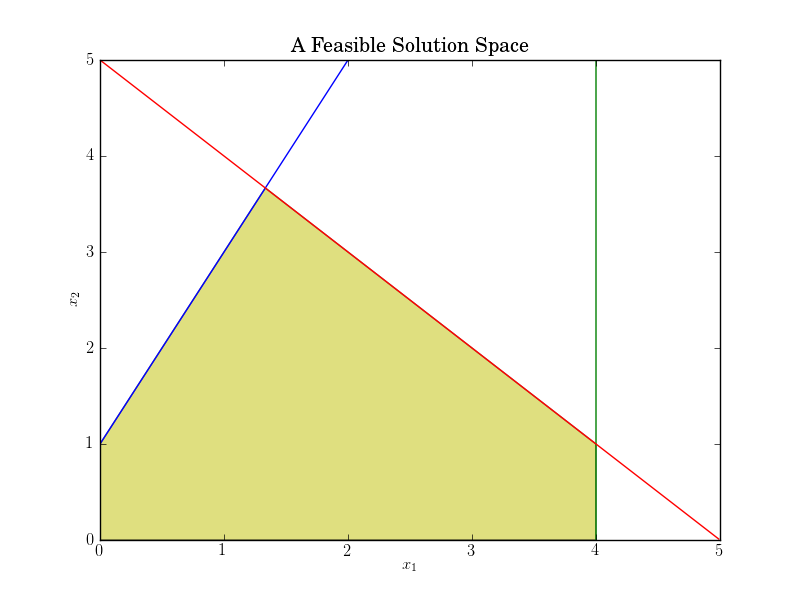
\includegraphics[width=\linewidth]{./chapters/litreview/plots/feasible.png}
  \caption{An example of a feasible solution space.}
  \label{fig:feasible}
  \end{center}
\end{figure}

The program can become infeasible by adjusting a constraint. Take for instance,
an increased boundary constraint for $x_2$.

%%% 
\begin{subequations}\label{eqs:infeas}
  \begin{align}
    %%
    \max \:\: & 
    3 x_1 + 2 x_2
    & \label{eqs:infeas_obj} \\
    %%
    \text{s.t.} \:\: &
    -2 x_1 + x_2 \leq 1 \\
    %%
    &
    x_1 + x_2 \leq 5 
    & \label{eqs:infeas_sup} \\
    %%
    &
    x_1 \in [0, 4]
    &\label{eqs:infeas_x1} \\
    %%
    &
    x_2 \geq 5
    &\label{eqs:infeas_x2}
    %%
  \end{align}
\end{subequations}
%%% 

This arrangement results in the infeasible linear program shown in
Figure \ref{fig:infeasible}, where the updated constraint's effect is shown in
red.

\begin{figure}[H]
  \begin{center}
    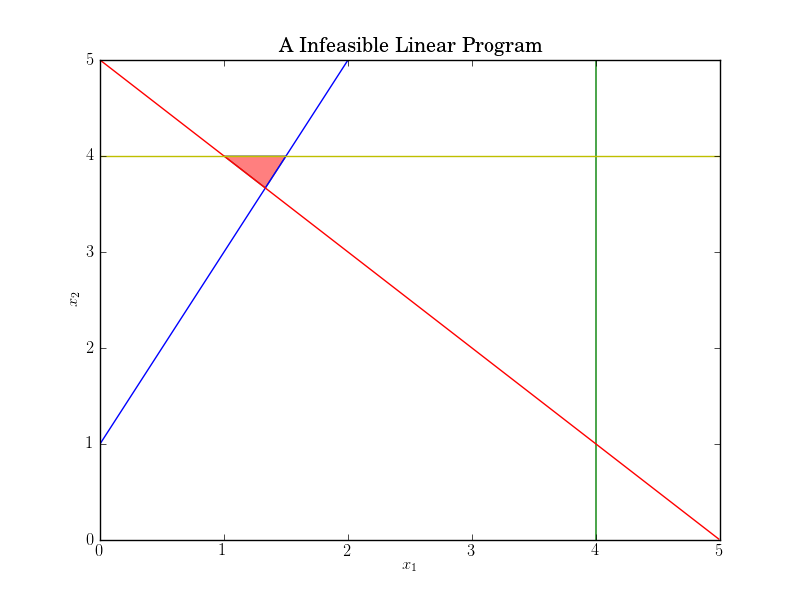
\includegraphics[width=\linewidth]{./chapters/litreview/plots/infeasible.png}
  \caption{An example of a infeasible solution space.}
  \label{fig:infeasible}
  \end{center}
\end{figure}

The standard form of a linear program shown in Equation \ref{eqs:std-form} is an
example of a \textit{primal} linear program. A distinction is made between
a \textit{primal} linear program and its \text{dual}. Duality theory is involved
and only treated lightly in this review. The standard form of the dual of
Equation \ref{eqs:std-form} is given in Equation \ref{eqs:dual-form}.

%%% 
\begin{subequations}\label{eqs:dual-form}
  \begin{align}
    %%
    \max_{u} \:\: & 
    w = b^{\top} u
    & \label{eqs:dual-form_obj} \\
    %%
    \text{s.t.} \:\: &
    A^{\top} u \leq c 
    & \label{eqs:dual-form_sup} \\
    %%
    &
    u \geq 0
    &\label{eqs:dual-form_x}
    %%
  \end{align}
\end{subequations}
%%% 

A few critical differences exist. First note that the objective directions are
switched: if a primal form has a minimization objective, its dual has a
maximization objective. The constraint matrix is now $M$ x $N$-dimensional (it
is in fact the original constraint matrix transposed). There is a new series of
decision variables that form the corresponding solution space, i.e., the
positive vector $u$, as shown in Equation \ref{eqs:dual-form_obj}. These
variables are related to the original right-hand side of the constraint
formulation, the vector $b$. The costs of the original problem, $c$, now form
the right-hand side of the dual's constraint formulation,
Equation \ref{eqs:dual-form_sup}.

The concept of duality is critical in the field of mathematical programming
because it provides well-defined optimality characteristics of a given
program. These are achieved via the \textit{Strong Duality Theorem}
and \textit{Weak Duality Theorem}, shown below as stated
in \cite{ferris_linear_2008}.

\begin{thm}[Weak Duality Theorem]
If $x$ is primal feasible and $u$ is dual feasible, then the dual objective
function evaluated at $u$ is less than or equal to the primal objective function
at $x$.
\end{thm}

The Weak Duality Theorem provides inextricable linkage between a primal feasible
solution and dual feasible solution. If a dual feasible solution is found, it
provides a lower bound on the optimal solution. If a primal feasible solution is
found, it provides an upper bound on the optimal solution. Both of these
criteria, in tandem, help to greatly reduce the required search space during
optimization sweeps.

\begin{thm}[Strong Duality Theorem]
Exactly one of the following three alternatives hold:
\begin{enumerate}

  \item Both primal and dual problems are feasible and consequently both have
  optimal solutions with \textit{equal} extrema

  \item \textit{Exactly one} of the problems is infeasible and consequently the
  other problem has and unbounded objective function in the direction of
  optimization on its feasible region

  \item \textit{Both} primal and dual problems are infeasible

\end{enumerate}
\end{thm}

The Strong Duality Theorem provides the backbone for much of linear programming
theory and application. It states that not only do feasible solutions to the
primal and dual programs provide upper and lower bounds on optimal values, but
that, in fact, the optimal values are \textit{equal}. This provides a criterion
to \textit{know} when an optimal value is reached.

With this slight overview of the realm of linear programming, one can move on to
solution techniques for problems that can be represented as linear programs.
\label{sec:lp-overview}

\subsection{The Simplex Algorithm}\label{sec:simplex}
\subsubsection{Overview}
The Simplex Method is a popular algorithm to solve linear programs first
published by Dantzig \cite{dantzig_maximization_1951}. Conceptually, it is quite
intuitive, especially from a geometrical point of view. I'll introduce the
method first in simple terms to provide a general idea before being a bit more
formal. Let us begin by discussing the example provided in the previous section.

We have the linear program:

%%% 
\begin{subequations}\label{eqs:lp}
  \begin{align}
    %%
    \max \:\: & 
    f(x_1, x_2) = 3 x_1 + 2 x_2
    & \label{eqs:lp_obj} \\
    %%
    \text{s.t.} \:\: &
    -2 x_1 + x_2 \leq 1 \\
    %%
    &
    x_1 + x_2 \leq 5 
    & \label{eqs:lp_sup} \\
    %%
    &
    x_1 \leq 4
    &\label{eqs:lp_x1} \\
    %%
    &
    x_1, x_2 \geq 0
    &\label{eqs:lp_x2}
    %%
  \end{align}
\end{subequations}
%%% 
 
Which appears geometrically as:

\begin{figure}[H]
  \begin{center}
    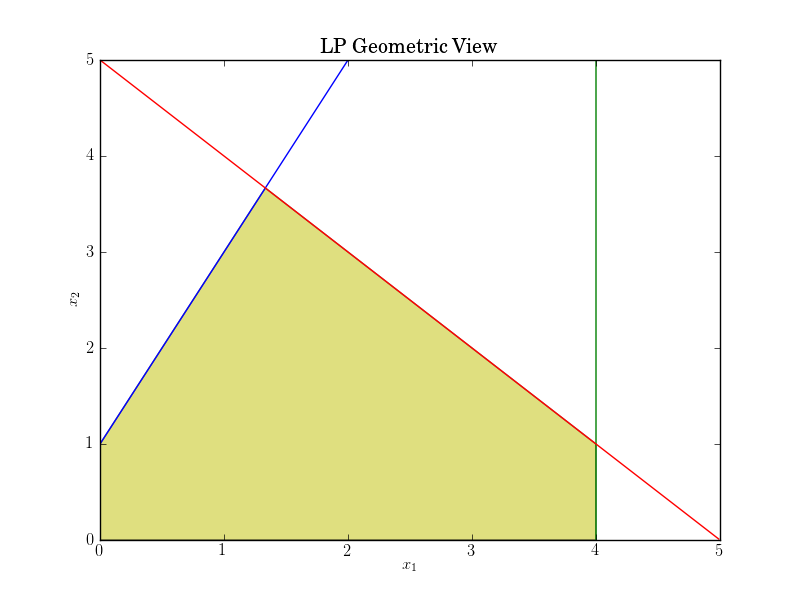
\includegraphics[width=\linewidth]{./chapters/litreview/plots/geometric.png}
  \caption{A Geometric View of the LP.}
  \label{fig:geometric}
  \end{center}
\end{figure}

Note that there are five vertices of the polygon (i.e., polytope) formed by the
full set of constraints:

\begin{enumerate}
  \item $(0, 0)$
  \item $(0, 1)$
  \item $(\frac{4}{3}, \frac{11}{3})$
  \item $(4, 1)$
  \item $(4, 0)$
\end{enumerate}

The Simplex Method begins at a vertex, for example $(0, 0)$, and evaluates the
objective function.

\begin{equation}
    f(0, 0) = 3 * 0 + 2 * 0 = 0 
\end{equation}

Neighbor vertices are then evaluated, in order to determine which provides the
larger value (in the case of maximizing objectives).

\begin{equation}
    f(0, 1) = 3 * 0 + 2 * 1 = 2 
\end{equation}

\begin{equation}
    f(4, 0) = 3 * 4 + 2 * 0 = 12 
\end{equation}

The vertex $(4, 0)$ provides a larger objective function value, so the algorithm
moves to this vertex and determines the next largest neighbor. In this simple
example, there is only one choice, and it is trivially larger.

\begin{equation}
    f(4, 1) = 3 * 4 + 2 * 1 = 14 
\end{equation}

Accordingly the algorithm moves a second time, analyzing the neighboring
vertices again.

\begin{equation}
    f(\frac{4}{3}, \frac{11}{3}) = 3 * \frac{4}{3} + 2 * \frac{11}{3} = \frac{34}{3} 
\end{equation}

At this last move, a terminating condition has been achieved: a vertex has been
found for which all of its neighbors provide a lower value for the objective
function, i.e.,

\begin{equation}
    14 \geq 12 \:\:\: \text{and} \:\:\: 14 \geq \frac{34}{3}.
\end{equation}

Thus, the optimal value for $(x_1, x_2)$ has been determined to be $(4, 1)$. It
is immediately obvious that the simplex algorithm in this state is a hill
climbing (or hill descending) algorithm. The chief reason why this is possible
(i.e., why one is guaranteed to find a globally optimum solution) is that the
objective function and constraints are \textit{convex} functions of the decision
variables. Convexification is a requirement for optimum solutions to both linear
and integer programs, and the tightest possible set of constraints for a given
program describes its \textit{convex hull}.

\subsubsection{In-Depth Discussion}
To begin a more robust discussion of the Simplex Method, one must introduce the
notion of \textit{slack variables}. Slack variables are used to transform
inequality constraints into equality constraints, effectively taking the
``slack'' out of the system. Slack variables are always positive, thus one could
use a slack variable, $s$, to convert

\begin{equation}
  \sum_{i} a_i x_i \leq b
\end{equation}

to 

\begin{equation}
  \sum_{i} a_i x_i + s = b
\end{equation}

and

\begin{equation}
  \sum_{i} a_i x_i \geq b
\end{equation}

to 

\begin{equation}
  \sum_{i} a_i x_i - s = b.
\end{equation}

The addition of slack variables allows one to rewrite an LP given in the
standard form of Equation \ref{eqs:std-form} as the \textit{canonical form}.

%%% 
\begin{subequations}\label{eqs:can-form}
  \begin{align}
    %%
    \min_{x, s} \:\: & 
    z =  c^{\top} x + 0^{\top} s
    & \label{eqs:can-form_obj} \\
    %%
    \text{s.t.} \:\: &
    A x - b = s
    & \label{eqs:can-form_sup} \\
    %%
    &
    x, s \geq 0
    &\label{eqs:can-form_x}
    %%
  \end{align}
\end{subequations}
%%% 

Given that there are $N$ decision variables and $M$ constraints, the cardinality
of $x$ is $N$ and the cardinality of $s$ is $M$. Furthermore, in these examples,
the $x_i$ variables are termed \textit{nonbasic} variables whereas the $s_i$
variables are termed \textit{basic} variables.

For any LP in the canonical form, the Simplex Algorithm can applied to it to
determine optimal values for its decision variables, or to determine that it is
unbounded or infeasible.

\begin{algorithm}[H]
 \SetAlgoLined
 \KwData{Decision variables, an objective function, and a set of constraints.}
 \KwResult{Optimal values for the decision variables or a flag denoting 
   infeasibility or unboundedness.}
 Get initial vertex\;
 \If{no vertex is found}{feasible solution space is empty}
  \While{not unbounded and not empty and not done}{ 
    Select column, i, via pricing\;
    \If{no column is found}{optimal condition found => done}
    Select row, j, via the ratio test\;
    \If{no row is found}{solution space is unbounded}
    Perform a Jordan exchange on element (i, j)\;
  }
  \caption{The Simplex Algorithm}
\end{algorithm}

There are four core operations associated with the Simplex Algorithm:
\begin{enumerate}
  \item finding an initial vertex
  \item column pricing
  \item row selection
  \item exchanging elements
\end{enumerate}

If finding an initial vertex is not trivial (e.g., if the origin is not a
candidate), then the operation to do so requires use of the Simplex Method on a
related LP where the origin is an available candidate. Accordingly, that process
will be described last.

The primary concept required to understand the Simplex Method's operations is
that of the \textit{basis}. The basis begins as the set of decision
variables. The algorithm progresses by moving slack variables into the basis,
and it does so efficiently by analyzing the most ``valuable'' variables to
target (i.e., which current basis variable affects the optimal value the most).

Column pricing and row selection are the operations that select the current
basis and nonbasis variables to target. The Jordan exchange actually performs
the translation of exchanging the basic and nonbasic variables. This is perhaps
more intuitive from a geometrical point of view. Consider some starting vertex
with many possible sides along which to move. The process of column pricing and
row selection \textit{chooses} the side along which to move, and the Jordan
exchange \textit{reorients} the problem. Revisiting the example problem,
remember the first step. The vertex $(4, 0)$ was determined to be the best
direction in which to move. After a Jordan exchange, the resulting LP would look
like Figure \ref{fig:rotated}.

\begin{figure}[H]
  \begin{center}
    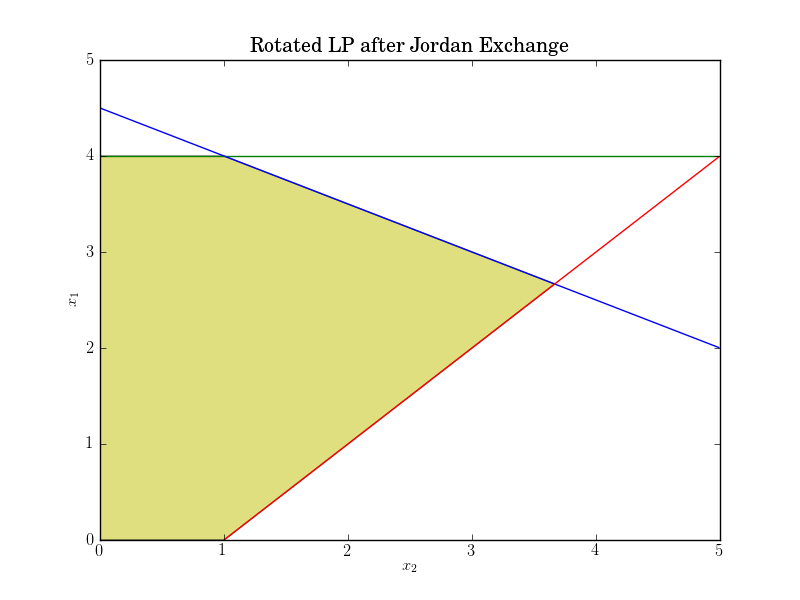
\includegraphics[width=\linewidth]{./chapters/litreview/plots/rotated.png}
  \caption{The Reoriented LP after the first Jordan Exchange.}
  \label{fig:rotated}
  \end{center}
\end{figure}

The column pricing operation selects the slack variable which will enter the
basis. The most naive implementation is to select the variable which will have
the largest effect on the objective function, i.e., which has the largest
magnitude \textit{reduced cost}. For instance, in Equation \ref{eqs:lp_obj},
$x_1$ has a reduced cost of 3, and $x_2$ has a reduced cost of 2 (note that both
costs are in the same positive direction as the objective, i.e.,
maximization). Accordingly, choosing $x_1$ as the nonbasic exchange variable is
a valid option. However, any algorithm may be used to make this selection, as
long as the reduced cost is positive.

Row selection, i.e., selecting the basic variable to enter the basis, is
performed via a ratio test. Given that a column $j$ has been selected, the
corresponding row, and thus basic variable, is selected according to
Equation \ref{eqs:ratio-max} in the case of a maximization objective and
Equation \ref{eqs:ratio-min} in the case of a minimization objective.

\begin{equation}\label{eqs:ratio-max}
  \min \left\{ \frac{-b_i}{A_{i,j}} \:\: | \:\: A_{i,j} > 0 \right\}
\end{equation}

\begin{equation}\label{eqs:ratio-min}
  \min \left\{ \frac{-b_i}{A_{i,j}} \:\: | \:\: A_{i,j} < 0 \right\}
\end{equation}

The Jordan Exchange operation, which transforms a matrix $A \mapsto A'$
given a pivot $(\hat{\imath}, \hat{\jmath})$, is straightforward and is shown in
Equation \ref{eqs:jordan}.

%%% 
\begin{subequations}\label{eqs:jordan}
  \begin{align}
    %%
    a_{\hat{\imath},\hat{\jmath}}' = \frac{1}{a_{\hat{\imath},\hat{\jmath}}}
    &\:\: \text{for} \:
    i = \hat{\imath}, j = \hat{\jmath} \\
    %%
    a_{\hat{\imath},j}' = -\frac{a_{\hat{\imath},j}}{a_{\hat{\imath},\hat{\jmath}}}
    &\:\: \text{for} \:
    i = \hat{\imath}, j \neq \hat{\jmath} \\
    %%
    a_{i,\hat{\jmath}}' = \frac{a_{i,\hat{\jmath}}}{a_{\hat{\imath},\hat{\jmath}}}
    &\:\: \text{for} \:
    i \neq i, j = \hat{\jmath} \\
    %%
    a_{i,j}' = a_{i,j} - a_{i,\hat{\jmath}} a_{\hat{\imath},j}
    &\:\: \text{for} \:
    i \neq \hat{\imath}, j \neq \hat{\jmath}
    %%
  \end{align}
\end{subequations}
%%% 

Finally, one must determine a starting vertex. The original linear program is
modified in the following way. For each row, $i$, if $b_i > 0$, then add an
additional variable, $x_0$ to the constraint with coefficient $a_i,0 = 1$. An
initial feasible point is then immediately available for $x = 0 \forall i \neq
0$ and $x_0 = \max(\max(b),0)$. The Simplex Method is then applied, with $x_0$
being the first variable to leave the basis. When $x_0$ returns to the basis, a
suitable starting vertex results from the removal of $x_0$.


\subsection{The Transportation Problem}\label{sec:xportation}
\subsubsection{Overview}
There are many canonical problems described in the linear programming
literature. A subset of these are classified as network flow programs, which are
ideal for modeling the flows between entities that comprise a model's
formulation. In computational science's parlance, entities make up a set of
nodes in a graph, and the possible connections between those entities make up
the arcs of a graph. Accordingly, if flow can occur between some node $i$ and
some other node $j$, then it flows along arc $(i, j)$. In general there is a set
of nodes $N$ and a set of arcs $A$, as shown in Figure
\ref{fig:node-arcs}. Decision variables in network flow problems determine the
optimal flow between nodes and across arcs.

\begin{figure}[H]
  \begin{center}
    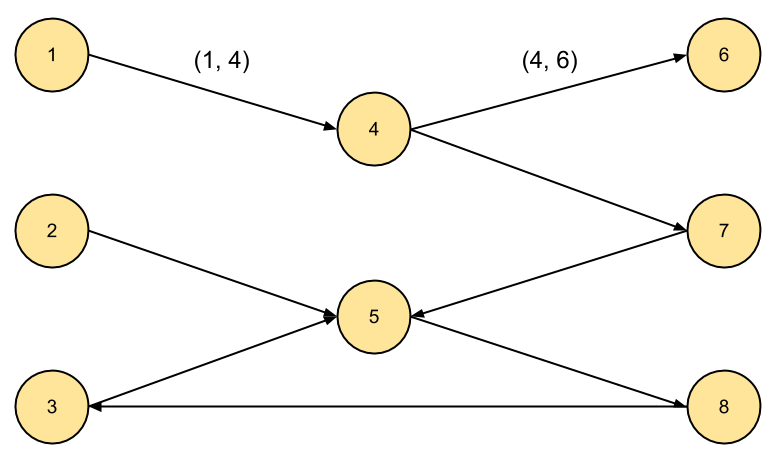
\includegraphics[height=7.5cm]{./chapters/litreview/node-arcs.png}
  \caption{An example node-arc network configuration. Arrows denote possible
    flow directions. Arc notation examples are provided for arcs (1,4) and
    (4,6).}
  \label{fig:node-arcs}
  \end{center}
\end{figure}

The actual formulation for a network flow problem as a linear program is, of
course, dependent on the problem being modeled. Take for example a maximum flow
problem. The objective of such a problem is to maximize the flow in a system,
i.e.,

\begin{equation}
\max \sum_{(i, j) \in A} x_{i,j}.
\end{equation}

The constraint matrix in such problems is denoted a \textit{node-arc incidence}
matrix. For a directed graph, an arc leaving node $i$ and entering arc $j$
indicates a value of 1 for element $a_{i,j}$ and a value of -1 for element
$a_{j,i}$. If an arc between two nodes does not exist, then a value of 0 is
assigned for the two corresponding coefficients. In general network flow
problems, there is also a notion of \textit{divergence}. Divergence is the total
amount of flow exiting or entering a node, and is modeled by the $b$ vector in
the matrix formulation of network flow problems. As is perhaps obvious, if $b_i
> 0$ for some node, $i$, then more flow exits the node than enters it and it is
termed a \textit{source node}. If $b_i < 0$, then more flow enters the node than
flows in, thus it is termed a \textit{sink node}. Finally, if $b_i = 0$, then
all material that flows into the node flows out as well, and it is termed a
\textit{transshipment node}. Finally, arcs can have their flow bounded, where a
lower bound for arc $(i, j)$ is given as $l_{i,j}$ and an upper bound is denoted
$u_{i,j}$.

One can now construct the LP formulation for a max-flow network flow problem.

%%% 
\begin{subequations}\label{eqs:max-flow}
  \begin{align}
    %%
    \max_{x} \:\: & 
    \sum_{(i, j) \in A} x_{i,j}
    & \label{eqs:max-flow_obj} \\
    %%
    \text{s.t.} \:\: &
    \sum_{j:(i,j) \in A} x_{i,j} - \sum_{i:(i,j) \in A} x_{i,j} = b_i
    & \forall i \in N \label{eqs:max-flow_sup} \\
    %%
    &
    l_{i,j} \leq x_{i,j} \leq u_{i,j}
    & \forall (i, j) \in A \label{eqs:max-flow_x}
    %%
  \end{align}
\end{subequations}
%%% 

\subsubsection{Transportation Problems}
Transportation problems are a subset of the network flow problems and can
therefore be modeled using linear programming. Transportation problems model the
flow of a commodity between source nodes and sink nodes, i.e., there are no
transshipment nodes in the general transportation problem. Critically, this
simplification allows for the nodes in the transportation problem to be
categorized into two explicit groups, sources and sinks. In other words, source
nodes and sink nodes comprise two distinct subsets, $N_1, N_2$, the union of
which comprises all nodes in the transportation graph, $N$. These properties can
be described in set notation.

\begin{equation}
  N_1 \subset N
\end{equation}

\begin{equation}
 N_2 \subset N
\end{equation}

\begin{equation}
  N_1 \cup N_2 = N
\end{equation}

From the node-arc graph point of view, this strict subset division allows for
the transportation problem to be modeled as a \textit{bipartite} graph.

\begin{figure}[H]
  \begin{center}
    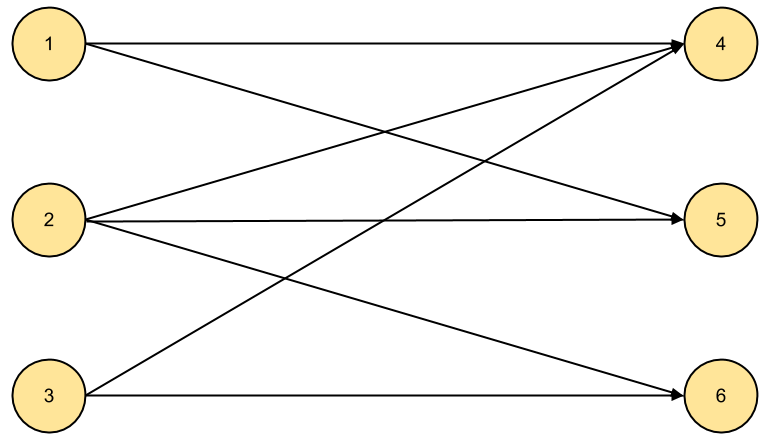
\includegraphics[height=7.5cm]{./chapters/litreview/node-arcs-bipartite.png}
  \caption{An example node-arc transportation network configuration. Arrows
    denote possible flow directions. Note that all nodes either belong to the 
    set of sources (left) or set of sinks (right).}
  \label{fig:node-arcs-bipartite}
  \end{center}
\end{figure}

The transportation problem is a platform on which one can model more general
problems. The minimum-cost transportation problem is a useful example. In such a
formulation, each arc has an associated \textit{unit cost} associated with the
cost of transporting a unit of a commodity along it, $c_{i,j}$. Additionally,
instead of the notion of divergence, supplier and consumer nodes have an
associated supply, $s_i$, or demand, $d_i$, which provide a notion
of \textit{node capacity} rather than arc capacity.

Accordingly, the minimum-cost transportation problem can be formulated as a
linear program in the following manner.

%%% 
\begin{subequations}\label{eqs:xport}
  \begin{align}
    %%
    \min_{x_{i,j}} \:\: & 
    \sum_{(i, j) \in A \subset N_1 \times N_2} c_{i,j} x_{i,j}
    & \label{eqs:xport_obj} \\
    %%
    \text{s.t.} \:\: &
    \sum_{j \in N_2} x_{i,j} \leq s_i
    & \forall i \in N_1  \\
    %%
    &
    \sum_{i \in N_1} x_{i,j} \geq d_i
    & \forall j \in N_2  \\
    %%
    &
    x_{i,j} \geq 0
    & \forall i \in N_1, \: \forall j \in N_2 \label{eqs:xport_x}
    %%
  \end{align}
\end{subequations}
%%% 

As is noted in many texts on the Transportation Problem Linear Program
formulation, an intuitive constraint on the problem to guarantee a feasible
solution is that the total demand in the system must be no greater than the
total supply in the system.

\begin{equation}
  \sum_{j \in N_2} d_j \leq \sum_{i \in N_1} s_i
\end{equation}

Feasibility in this sense can be guaranteed, however, by adding an artificial
supply node. Such a node can have infinite supply capacity but at (effectively)
infinite cost. The problem can then be solved, and any flow leaving the
artificial node in the optimal solution can be dealt with accordingly, e.g., it
can be ignored.

\subsubsection{Multi-Commodity Transportation Problems}\label{sec:MCTP}
The previously-described transportation problem can more precisely be named the
single-commodity transportation problem. It deals with the flow from sources to
sinks of a single commodity. A more complex model includes more than one
commodity.

Variables and constants in the multi-commodity formulation are generally analogs
of their counterparts in the single-commodity problem. There is a unit cost for
commodity $h$ to traverse arc $(i,j)$ denoted as $c_{i,j}^{h}$. A supplier of
commodity $h$ has a certain supply capacity $s_i^h$ which cannot be surpassed
and demanders of commodity $h$ have a certain demand level which must be met,
$d_i^h$.

In the simplest extension from the single-commodity to multi-commodity
transportation problem, arc constraints for all commodities are combined, i.e.,
for a given arc $(i, j)$, there is a single capacity $u_{i,j}$. A classic
interpretation of this enhanced complexity deals with data networks. Multiple
classifications of data exist, but they all must traverse the same network
infrastructure. Accordingly, the infrastructure can only accommodate a certain
level of total flow among all communication types.

This coupling of commodities via arc capacities changes the structure of the
node-arc incidence matrix. Arc capacity constraints no longer have a single
entry. Instead, many flows contribute to the capacity constraint, requiring
different methods to solve the problem. Of course, the Simplex Method can still
solve the linear program, however other potential reductions in time and
complexity that are available to the single-commodity flow problem are not
available to the multi-commodity flow problem due to this coupling.

The formulation of the multi-commodity flow problem is shown in Equation
\ref{eqs:MCTP}. Note the commodity coupling in Equation \ref{eqs:MCTP_cap}.

%%% 
\begin{subequations}\label{eqs:MCTP}
  \begin{align}
    %%
    \min_{x_{i,j}^{h}} \:\: & 
    \sum_{i \in I}\sum_{j \in J}\sum_{h \in H} c_{i,j}^{h} x_{i,j}^{h}
    & \label{eqs:MCTP_obj} \\
    %%
    \text{s.t.} \:\: &
    \sum_{j \in J} x_{i,j}^{h} \leq s_{i}^{h}
    &
    \forall \: i \in I, \forall \: h \in H \label{eqs:MCTP_sup} \\
    %%
    &
    \sum_{i \in I} x_{i,j}^{h} \geq d_{j}^{h}
    & 
    \forall \: j \in J, \forall \: h \in H \label{eqs:MCTP_dem} \\
    %%
    &
    \sum_{h \in H} x_{i,j}^{h} \leq u_{i,j}
    & 
    \forall \: j \in J \label{eqs:MCTP_cap} \\
    %%
    &
    x_{i,j}^{k} \geq 0
    &
    \forall \: i \in I, \forall \: j \in J, \forall \: h \in H \label{eqs:MCTP_x}
    %%
  \end{align}
\end{subequations}
%%% 

A number of important reductions are possible for the multi-commodity
transportation problem, e.g., the case in which is no arc that shares multiple
commodities. In this instance the multicommodity connection constraints
disappear, and the single multi-commodity problem can be broken into $m$
different single-commodity transportation problems, where $m$ is the cardinality
of the set of commodities, $H$. 


\subsection{The Multicommodity Transport Problem}\label{sec:MCTP}
\input{./chapters/litreview/mc-xportation}

%%% 
\begin{subequations}\label{eqs:MCTP}
  \begin{align}
    %%
    \min_{z} \:\: & 
    z = \sum_{i \in I}\sum_{j \in J}\sum_{h \in H} c_{i,j}^{h} x_{i,j}^{h}
    & \label{eqs:MCTP_obj} \\
    %%
    \text{s.t.} \:\: &
    \sum_{j \in J} x_{i,j}^{h} = a_{i}^{k}
    &
    \forall \: i \in I, \forall \: h \in H \label{eqs:MCTP_sup} \\
    %%
    &
    \sum_{i \in I} x_{i,j}^{h} = b_{j}^{k}
    & 
    \forall \: j \in J, \forall \: h \in H \label{eqs:MCTP_dem} \\
    %%
    &
    \sum_{h \in H} x_{i,j}^{h} \leq u_{i,j}
    & 
    \forall \: j \in J \label{eqs:MCTP_cap} \\
    %%
    &
    x_{i,j}^{k} \geq 0
    &
    \forall \: i \in I, \forall \: j \in J, \forall \: h \in H \label{eqs:MCTP_x}
    %%
  \end{align}
\end{subequations}
%%% 

\subsection{The Linear Approximation Model}\label{sec:approx}
Another application of linear programming involves approximating solutions to
linear systems of equations in the form of Equation \ref{eqs:lin-sys}.

\begin{equation}\label{eqs:lin-sys}
A x = b
\end{equation}

$A$ is an $m x n$-dimensional constraint matrix that can
be \textit{overdetermined}, i.e., include more constraints than decision
variables. Given some approximation of the solution, $\tilde{x}$, one can define
the residual, $r$, associated with that approximation.

\begin{equation}\label{eqs:lin-sys}
A \tilde{x} - b = r
\end{equation}

One can then formulate an optimization problem that seeks to minimize the
$\ell_p$-norm of the residual vector, $r$. The literature treats three types of
norms, $\ell_1$, $\ell_2$, and $\ell_\infty$, where each can be defined as
follows.

\begin{equation}
\ell_1 (r) = \| r \|_1 = \sum_{i = 1}^{m} | r_i |
\end{equation}

\begin{equation}
\ell_2 (r) = \| r \|_2 = \sqrt{ \sum_{i = 1}^{m} | r_i |^2 }
\end{equation}

\begin{equation}
\ell_\infty (r) = \| r \|_\infty = \max_{i} | r_i |
\end{equation}

The linear programming formulation takes as its minimizing function the
residual, for which individual $x_i$ values form the decision
variables. Accordingly, each $\ell_p$ norm formulation is slightly
different. 

The $\ell_\infty$ norm utilizes a maximum-violation variable $\epsilon$, as shown
in Equation \ref{eqs:l-inf}.

%%% 
\begin{subequations}\label{eqs:l-inf}
  \begin{align}
    %%
    \min \:\: & 
    \epsilon  \\
    %%
    \text{s.t.} \:\: &
    - \epsilon \leq A_i x - b_i
    & \forall i \\
    %%
    &
    \epsilon \geq A_i x - b_i
    & \forall i \\
    %%
  \end{align}
\end{subequations}
%%% 

The $\ell_1$ norm uses a summation over all violations, as shown in
Equation \ref{eqs:l-1}, by using a proxy vector, $y$.

%%% 
\begin{subequations}\label{eqs:l-1}
  \begin{align}
    %%
    \min \:\: & 
    \sum_i y
    & \\
    %%
    \text{s.t.} \:\: &
    - y_i \leq A_i x - b_i
    & \forall i \\
    %%
    &
    y_i \geq A_i x - b_i
    & \forall i \\
    %%
  \end{align}
\end{subequations}
%%% 

The core difference between the two formulations is of course the norm used. The
$\ell_1$ norm in this case stores more information about the total violation,
whereas the $\ell_\infty$ norm is concerned with only the largest violating
constraint. These formulations are easily solved by the Simplex Method, as a
starting vertex can always be chosen by setting $x = 0$.

The $\ell_2$ norm is not as straightforward to solve. As shown
in \ref{ferris_linear_2008}, the actual norm can be replaced by its square,
because it is uniformly nonnegative. The resulting optimization problem is shown
in Equation \ref{eqs:l-2}.

%%% 
\begin{subequations}\label{eqs:l-2}
  \begin{align}
    %%
    \min \:\: & 
    y^\top y
    & \\
    %%
    \text{s.t.} \:\: &
    - y_i \leq A_i x - b_i
    & \forall i \\
    %%
    &
    y_i \geq A_i x - b_i
    & \forall i \\
    %%
  \end{align}
\end{subequations}
%%% 

As can be seen in its formulation in Equation \ref{eqs:l-2}, the objective
function is not a linear function of the decision variables. Accordingly, one
must tackle this problem using a different domain of mathematical programming,
namely \textit{quadratic programming}, the discussion of which is outside the
scope of this review due to the lack of its necessity to adequately solve the
Recipe Approximation Problem described in \S\ref{sec:rap}.


\section{Integer Programming}\label{sec:ip}

\subsection{The Branch and Bound Algorithm}\label{sec:bnb}

\chapter{Previous Work}\label{ch:prevwork}

The previous work I've completed has focused primarily on efforts to run and
benchmark simple, once-through fuel cycle simulations with \Cyclus. Supporting
this effort has required not only additions to the \Cyclus code base to model
enrichment and reactor facilities, but also to the peripheral (i.e., linking
and input/output) and simulation-related infrastructure.

Significant, strategic improvements have been added to the \Cyclus code base
regarding interactions with dynamically-loadable libraries and reading XML-input
files. Basic simulation setup and execution has been revised to provide clear
phases of initialization. Tools have also been added to provide agent-based
management of building and instantiation of child agents, i.e., facilities in the
\Cyclus simulation. A (currently) separate library, named \Cyclopts, has been
developed to provide an interface to optimization solvers which currently
supports COIN-OR's linear and integer program solvers
\cite{lougee_common_2003}. Management of the actual building (instantiation) of
facilities within the simulation framework has been encapsulated in a
supplier/manager class pair. Finally, additional support has been added
specifically regarding to model enrichment-related calculations, allowing for
enrichment facilities to be developed in \Cycamore.

The combination of the above enhancements, in addition to developing an
enrichment and batch-based reactor facility models, as well as a managerial
institution model and demand-based region model, resulted in a \Cyclus
once-through fuel cycle simulation. In order to benchmark the basic simulation
infrastructure, the INPRO \cite{_international_2009} once-through benchmark was
used and compared with results from the VISION \cite{yacout_vision_2006}
code. Output closely matched for both reactor growth, gross material flows, and
SWUs utilized. Discrepancies were seen for the amount of natural uranium
utilized. The exercise of developing an input file for the the benchmark
specification was tedious due to the lack of published specifications. After a
review of other benchmarks, this was shown to be a common problem in addition to
a general lack fully specifying benchmark scenarios. Accordingly, a new
specification language was proposed and implemented, and a translation package
was implemented in order to translate that input into a \Cyclus input file.

\section{\Cyclus To Date}

\subsection{Dynamic Loading}\label{sec:prev-dynamic}

Libraries can be accessed in a static manner, i.e., they are connected to an
application during the linkage phase, or can be accessed in a dynamic manner,
i.e., they are connected at run time. Dynamic linkage, or dynamic loading, is a
well-known technique for to support connectable, modular components, or
plug-ins. \Cyclus utilizes a plug-in approach for its facility, institution, and
region agents. This design decision furthers the \Cyclus development goal of
providing an agnostic framework into which sophisticated users can develop
different models of agents to investigate a certain simulation-modeling change.

Work was performed in order to use class-based representation of dynamic
libraries, allowing for easy opening, closing, and access thereof. Each dynamic
library represents an agent type in \Cyclus, providing a constructor and
destructor. The DynamicModule class then provides the \Cyclus Core access to
these constructors and destructors to perform the appropriate operations at run
time. Because dynamic loading is treated differently on POSIX-based systems than
it is on Windows-based systems, specialty functions for library access were
provided for each system. The correct header file (UnixHelperFunctions.h or
WindowsHelperFunctions.h) is chosen during compilation. 

These changes simplified the client code that utilizes library access. The
\Cyclus Core application can now call appropriate library-related functions in
an agnostic manner. Specific, well-defined time points of module loading
(dynamic library opening) and unloading (dynamic library closing) were defined
in the \Cyclus application. These operations, called by the application,
currently reside in the Model class and could likely be refactored into a
specific handler class designed for this purpose.

\subsection{Input Reading}

A large overhaul to the input-reading code base was performed. \Cyclus currently
only supports XML input files that adhere to the RNG schema defined in \Cyclus
RNG file. However, it is a well-known best practice to provide an agnostic
application programming interface (API) that can be configured with specific
instances given some user-defined input. Accordingly, such an API was
constructed which currently supports XML input but can also support future input
types that are tree-based (e.g., JSON, CSV, etc.).

The top-level abstraction is encased in a QueryEngine class. Basic operations
are provided assuming a tree-based input formation, including querying the
number of child elements at the current reading level, the name of each element,
and access to each element. The application code is responsible for configuring
the appropriate input parser and populating an instance of a QueryEngine at its
root. The client code then populates input parameters through the QueryEngine
interface rather than an input-format specific interface.

Support for XML-file reading has been enhanced by separating various concerns
into appropriate classes. Four classes have been constructed with specific
purposes regarding input file reading: file loading (XMLFileLoader), file
validation (RelaxNGValidator), file parsing (XMLParser), and querying
(XMLQueryEngine). The application interfaces with the file loader, initializing
it with a given input file path and then invoking the loading of various
\Cyclus-specific parameters (e.g., simulation control parameters, material
recipes, agent modules, etc.). The loader is responsible for managing its parser
and providing client code with correctly-configured instances of
XMLQueryEngines. The parser is responsible for providing an interface to the
underlying C++ XML parsing library (currently libxml++ is used) and invoking the
appropriate validation routines on the parsed file. The validator is responsible
for providing access to the RNG-validation operations through, currently, libxml
and libxml++. Finally, the XML-specific derived QueryEngine class is responsible
for implementing XML-specific querying using the generic QueryEngine interface.

Other input file formats can be supported by providing the appropriate
format-specific derived QueryEngine class and adjusting the application code as
necessary. To developer could then choose how to implement the loading and
validation, if any, of the input file. The above structure is just one of many
ways to achieve such a goal.

\subsection{Enrichment Tools}\label{sec:prev-enrich}

The ability to calculate enrichment-related values is required to provide
important metrics for the simplest of fuel cycle simulations. Enrichment is the
process of artificially increasing the relative amount of Uranium-235 in a given
sample of Uranium. Naturally, Uranium contains approximately 0.72\% U-235, a
small amount (~0.005\%) U-234, and 99.274\% U-238. In light-water reactors
(LWRs), fissile U-235 is the primary fission fuel source, and thus reactors run
longer with higher amounts of U-235. Accordingly, reactor fuels are enriched to
~3-6\% U-235. It should be noted that enrichment of Uranium above 20\% is
restricted by international law due to its capacity to be used as a weapon in
high concentrations. In practice, however, Uranium-based nuclear weapons
generally have enrichments of greater than 90\%.

The enrichment process has one input, or feed, stream (usually natural Uranium)
and two output streams, the product and the excess Uranium, called tails. The
U-235 abundance, or assay of each of these streams as well as the mass of each stream
determines how much work is required to perform the enrichment, where
enrichment-work is calculated using Separative Work Units (SWUs). The feed,
product, and tails stream mass and assay values are related. Equation
\ref{eqs:enr-feed} shows the relation between product and feed masses, and
Equation \ref{eqs:enr-tails} shows the relation between product and tails
masses. 

\begin{equation}\label{eqs:enr-feed}
  F = P \frac{x_{p} - x_{t}}{x_{f} - x_{t}}
\end{equation}

\begin{equation}\label{eqs:enr-tails}
  T = P \frac{x_{p} - x_{f}}{x_{f} - x_{t}}
\end{equation}

Note that both equations depend on the U-235 assay ($x_i$s) of each
stream. Furthermore, given the assay of each stream, one needs to either set
the product or feed value (in the case of Equation \ref{eqs:enr-feed}) and the
product or tails value (in the case of Equation \ref{eqs:enr-tails}). In
practice, the feed and tail assays are set and an order for some quantity of
enriched product is requested. The resulting required feed and tail masses are
then calculated.

Enrichment plants measure their production in SWUs due to the quality
(enrichment level) variation of their product from order to order. The amount of
SWUs required to enrich a quantity of Uranium to a certain assay is a
function of all of the aforementioned variables (assays and masses of the
feed, product, and tails streams). The SWU calculation is shown in Equation
\ref{eqs:enr-swu}, where $V(x)$ is the Value Funtion defined in Equation
\ref{eqs:enr-value}.

\begin{equation}\label{eqs:enr-swu}
  SWU = P \; V(x_{p}) + T \; V(x_{t}) - F \; V(x_{f})
\end{equation}

\begin{equation}\label{eqs:enr-value}
  V(x) = (1 - 2x) \ln \left( \frac{1-x}{x} \right)
\end{equation}

Combining Equations \ref{eqs:enr-feed}, \ref{eqs:enr-tails}, and
\ref{eqs:enr-swu}, one can represent the SWU calculation as a function only of
the product mass and feed, product, and feed stream assays as shown in
Equation \ref{eqs:enr-swu-p}.

\begin{equation}\label{eqs:enr-swu-p}
  SWU = P \left( V(x_{p}) + \frac{x_{p} - x_{f}}{x_{f} - x_{t}} V(x_{t}) 
        - \frac{x_{p} - x_{t}}{x_{f} - x_{t}} V(x_{f}) \right)
\end{equation}

An Enrichment class was added to the \Cyclus set of utility toolkits under the
enrichment namespace. A simple Assay container class was also added, and is used
as the argument to many of the above calculations. The Enrichment toolkit allows
for the calculation of each of the abovementioned values and is used primarily
in the EnrichmentFacility that was added to \Cycamore to run the once-through
fuel cycle benchmarks.

\subsection{Facility Building and Supply/Demand Tools}

In order to support simple, once-through fuel cycle simulations, a nominal
capacity supply-demand interaction capability was needed. The use case of such a
system is to define demand for a given installed capacity, say in gigawatts of
produced power. Agents in a \Cyclus simulation generally have a natural
lifecycle, leaving the simulation at the end of their lifetimes. The system must
be able to respond to changes in installed capacities if it is to continue to
meet the simulated demand curves.

\subsubsection{Facilities as Prototypes}
After reviewing the prior status of the code base and the way in which
Facilities were being defined and instantiated, I noted that there was not a
well-formed entry or exit point for facilities in the simulation
infrastructure. Accordingly, I updated the methodlogy behind such operations to
use the Prototype design pattern \cite{vlissides_design_1995}. A prototype is a
creational pattern that keeps a prototypical instance of an object
available. When a new instance is required, a copy of this prototypical instance
is made and returned. This strategy fit naturally with the \Cyclus input format
and code base. Nominal paramters defining ``classes'' of facilities, e.g. a
certain type of reactor or supporting facility, are listed in XML input
files. The code base has been updated to create prototypical instances of each
facility defined in the input file during a simulation initialization step. When
a new facility is required to be built in the simulation, a copy of a prototype
is introduced.

\subsubsection{Symbolic Functions}

The ability to represent symbolic functions was added to the \Cyclus Utiliy
toolkit. Functions are represented by a base Function class providing an
appropriate API. Linear, exponential, and piecewise function classes are
supported, where piecewise functions can utilize both linear and exponential
piecewise functions. Factory classes are provided to take a string of parameters
as read from an input file and return the appropriate symbolic function. A
simple example of the piecewise function support is provided in Figure
\ref{fig:piecewise}.

\begin{figure}[H]
  \begin{center}
    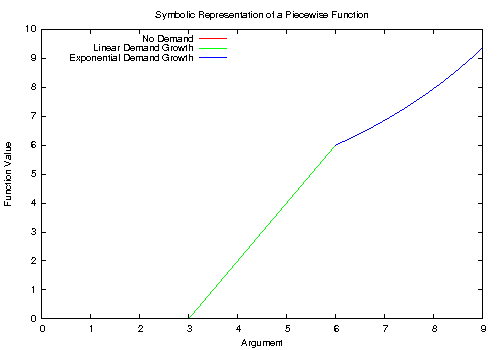
\includegraphics[width=\linewidth]{./chapters/prevwork/piecewise.png}
  \caption{An example of a piecewise function represented using the updated API.}
  \label{fig:piecewise}
  \end{center}
\end{figure}

\subsubsection{Tracking Commodity Production Capacity}

There is a need to track the current capacity of the production of a certain
commodity. Electrical power was offered the a prime example for this
once-through fuel cycle use case. Accordingly, a simple ``mixin'' class
\cite{ulrich_mixin-based_2001} called CommodityProducer was developed. It offers
an interface for accessing a list of commodities an entity produces and their
associated capacity to produce each commodity as well as the unit price of
commodity production. To date, the mixin has been used in conjunction with the
BatchReactor class, which serves as the reactor model for the once-through fuel
cycle simulations. The BatchReactor subclasses from both the base Facility class
as well as the CommodityProducer class.

A CommodityProducerManager class was also developed to manage a collection of
commodity producers. Its interface include registration and unregistration
methods to keep track of the producers it manages as well as a simple interface
for querying the current total capacity level of the commodity producers it
manages. It is also designed as a ``mixin'' class which has been utilized by the
ManagerInst class in \Cycamore, allowing the institution to keep track of the
capacity of facilities that produce certain commodities (e.g., electrical
power). This manager class is a use of the classic Observer design pattern
\cite{vlissides_design_1995}.

\subsubsection{Supply/Demand Tracking and Intelligent Build Decisions}

Three concerns remain in order to implement an appropriate model of responses to
changing supply capacity and demand for capacity. First, the current supply and
demand levels must be queryable. Second, if demand is greater than supply, some
new simulation entity must be built or introduced into the simulation. Third, a
decision must be made as to which entities should be built to meet a demand gap
if it exists.

A SupplyDemandManager class has been introduced to provide an interface for
querying the current supply capacity and demand for a given commodity. The class
is an Observer of CommodityProducerManagers, querying them when appropriate to
determine the full production capacity for the union of CommodityProducers
managed by the set of CommodityProducerManagers. Demand functions are also
registered for each commodity. An instance of a SupplyDemandManager is a private
member of the GrowthRegion class in \Cycamore, which supports building
facilities based on user-defined growth curves.

A Builder class has been introduced an interface for an entity that can build,
or instantiate into the simulation, instances of CommodityProducers. It is
designed as a ``mixin'' class and is utilized by the ManagerInst class in
\Cycamore. To date, institutions have been thought of as managers of facilities
by the \Cyclus development team, thus it is possible that the notion of facility
deployment management encapsulated in the current version of the ManagerInst
could be refactored into the Institution base class in the \Cyclus core
database. Such a decision will be informed by present and future use cases.

Finally, the BuilderManager class has been introduced to encapsulate the
decision making operations regarding building new facilities. It is an Observer
of Builder class instances, and an instance of the BuilderManager is used as a
private member by the GrowthRegion class in \Cycamore. The BuilderManager
interacts with the region's SupplyDemandManager to query the existence of unmet
demand. If it exists, it solves an integer program formulated as Equation
\ref{eqs:build-decision},

%%% 
\begin{subequations}\label{eqs:build-decision}
  \begin{align}
    %%
    \min \:\: & 
    \sum_{f \in F} n_f c_f
    & \\
    %%
    \text{s.t.} \:\: &
    \sum_{f \in F} n_f \phi_f \ge \Phi
    & \\
    %%
    &
    n_f > 0 \: \text{and} \: integer
    &
    \forall f \in F
    %%
  \end{align}
\end{subequations}
%%% 
  
where $\Phi$ is the unmet demand, $F$ is the set of facilities capable of
meeting the demand, and, for each facility in $F$, $c_f$ is the cost of
building, and $\phi_f$ is the nameplate capacity.  Finally, $n_f$ is the
optimized number of facilities to build of type $f$. The set of facilities and
their associated costs and capacities are queried through the managed Builder
instances.

\subsection{\Cyclopts}

Proposed in this thesis and already implemented in the \Cyclus code base is a
heavy usage of integer and linear programming. The domain of mathematical
programming is well studied and many LP, IP, MILP solvers exist. The majority of
solvers or codes supporting such solvers are closed source (e.g., BARON, CPLEX,
Maple, MATLAB, etc.). Such programs are generally faster than their open source
cousins, but are restrictive to use in implementation of an open source library
like \Cyclus. Accordingly, there is a use case for providing an abstract
interface for defining mathematical programs that can support concrete
implementations based on the library used.

\Cyclopts has been developed as a separate library to provide such an
interface. Basic constructs such as variables, functions, and solvers are all
represented as concrete classes. Different solver libraries are implemented by
deriving from the base Solver class. An interface class is provided to connect
abstract concepts required to define a problem instance with a concrete solver.

Currently, COIN-OR's Coin-Branch-and-Cut (CBC) \cite{lougee_common_2003} solver
is supported as a proof of principle. The \Cyclopts library is used by the
BuilderManager class in \Cyclus to determine the solution of Equation
\ref{eqs:build-decision}. Future development will include adding a full test
suite to \Cyclopts and integrating it as a part of the \Cyclus core as
additional use cases present themselves. Such cases will arise through the
implementation of this thesis.

\section{Benchmarking Efforts}\label{sec:prev-benchmark}

As with any code base, validation and verification (V \& V) exercises are
critical to have confidence in the answers provided by the code. Fuel cycle
simulators are an interesting V\&V case in that they model proposed future cases
of nuclear fuel cycles, effectively predicting 

blah blah revisit.

\subsection{VISION Once-Through}

The \Cyclus core and \Cycamore modules were used to conduct a benchmark
comparison with VISION, a fuel cycle code developed in PowerSim and Excel by the
Idaho National Laboratory. A single case was compared, 

blah blah revisit.

% reactors
\begin{figure}[H]
  \centering
  \subfloat[Low Case]{%
    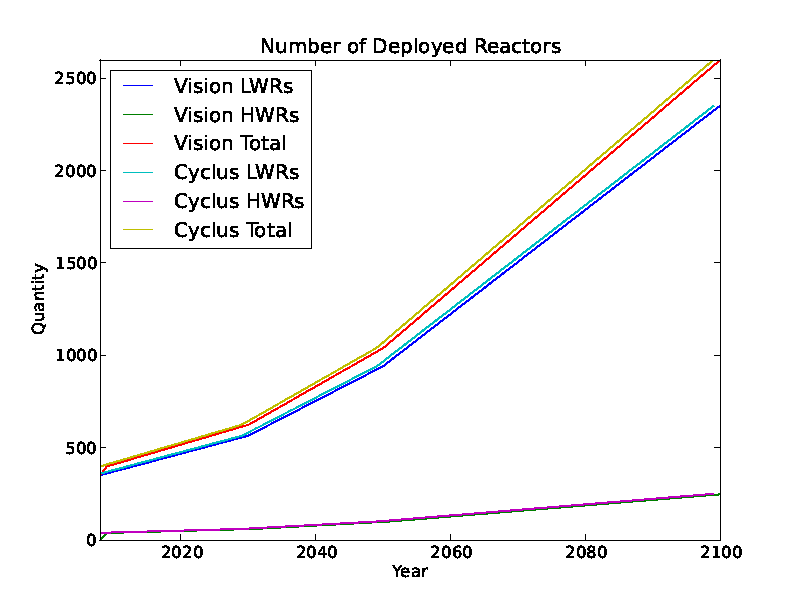
\includegraphics[width=.45\linewidth]{./chapters/prevwork/graphs/rxtrs_low.png}
    \label{fig:rxtrs_low}}
  \quad
  \subfloat[High Case]{%
    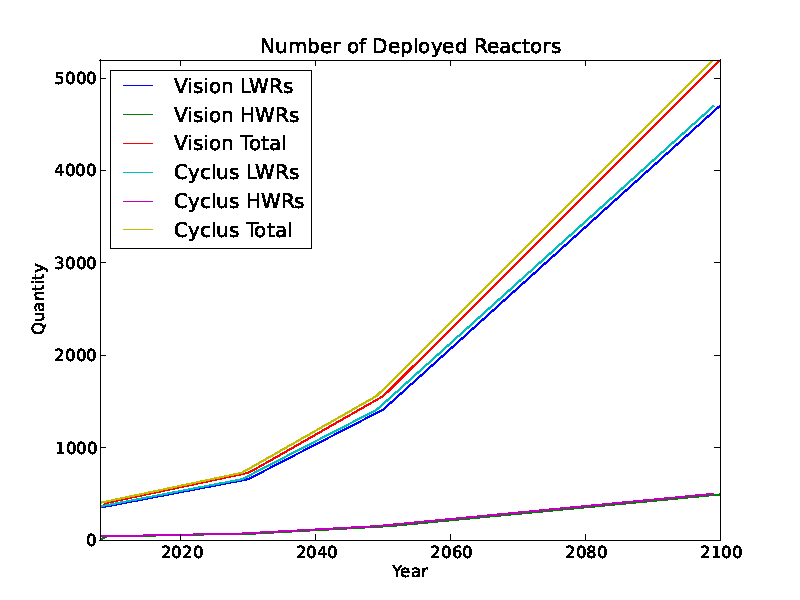
\includegraphics[width=.45\linewidth]{./chapters/prevwork/graphs/rxtrs_high.png}
    \label{fig:rxtrs_high}}
\caption{Reactors built in each INPRO demand case.}
\label{fig:rxtrs}
\end{figure}

% used fuel
\begin{figure}[H]
  \centering
  \subfloat[Low Case]{%
    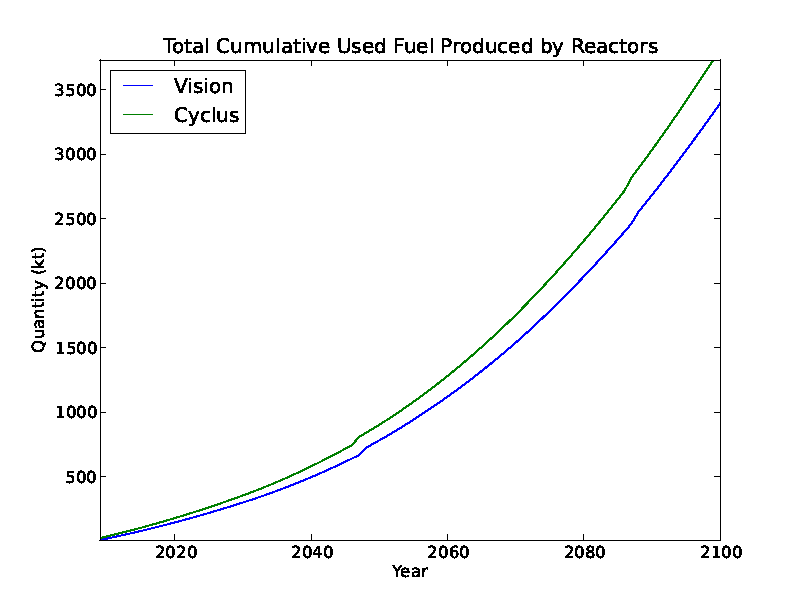
\includegraphics[width=.45\linewidth]{./chapters/prevwork/graphs/used_fuel_low.png}
    \label{fig:used_fuel_low}}
  \quad
  \subfloat[High Case]{%
    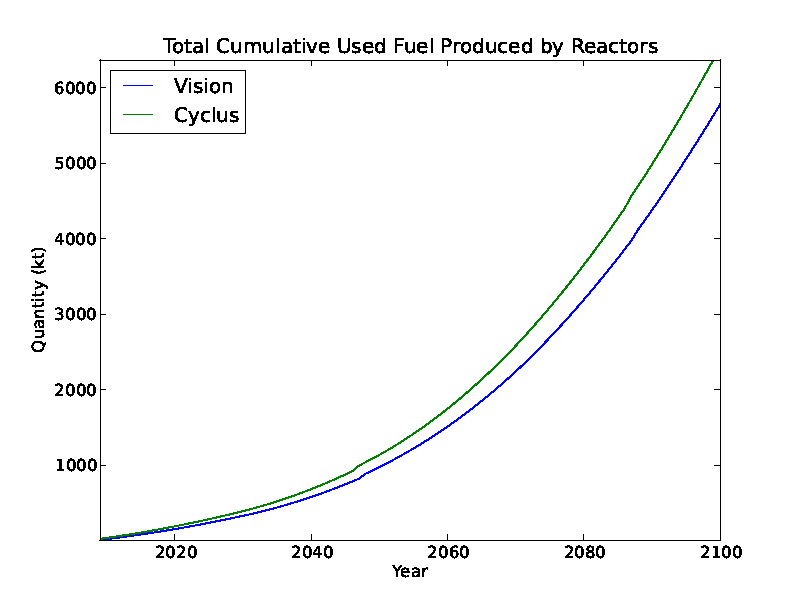
\includegraphics[width=.45\linewidth]{./chapters/prevwork/graphs/used_fuel_high.png}
    \label{fig:used_fuel_high}}
\caption{Used fuel exiting reactors in each INPRO demand case.}
\label{fig:used_fuel}
\end{figure}

% nat u
\begin{figure}[H]
  \centering
  \subfloat[Low Case]{%
    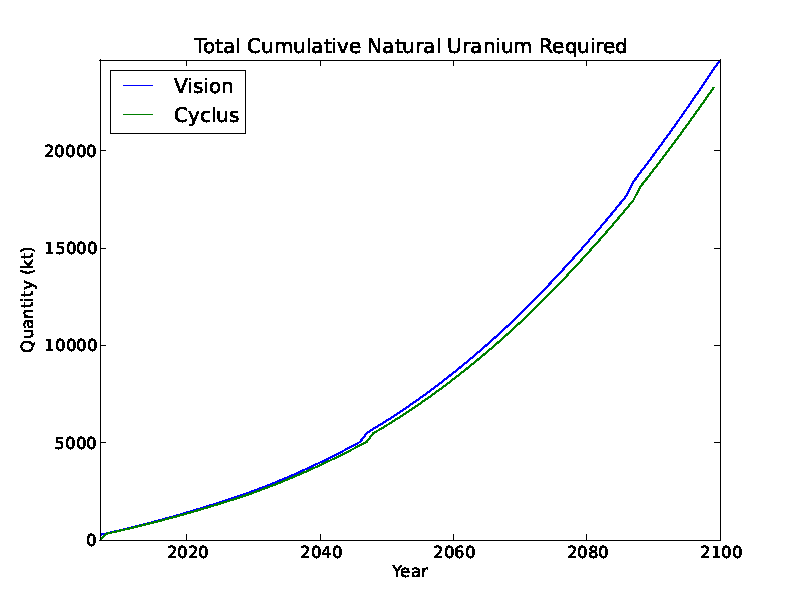
\includegraphics[width=.45\linewidth]{./chapters/prevwork/graphs/nat_u_low.png}
    \label{fig:nat_u_low}}
  \quad
  \subfloat[High Case]{%
    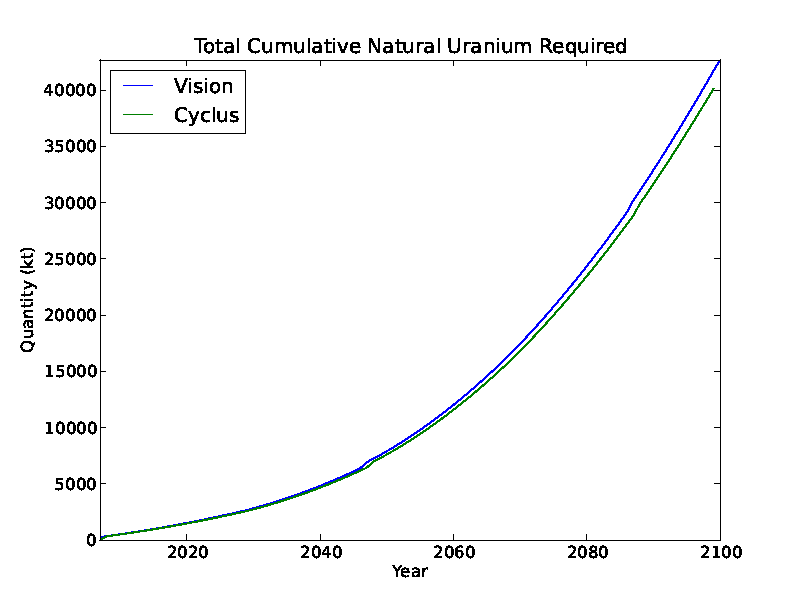
\includegraphics[width=.45\linewidth]{./chapters/prevwork/graphs/nat_u_high.png}
    \label{fig:nat_u_high}}
\caption{Natural uranium usage in each INPRO demand case.}
\label{fig:nat_u}
\end{figure}

% swu
\begin{figure}[H]
  \centering
  \subfloat[Low Case]{%
    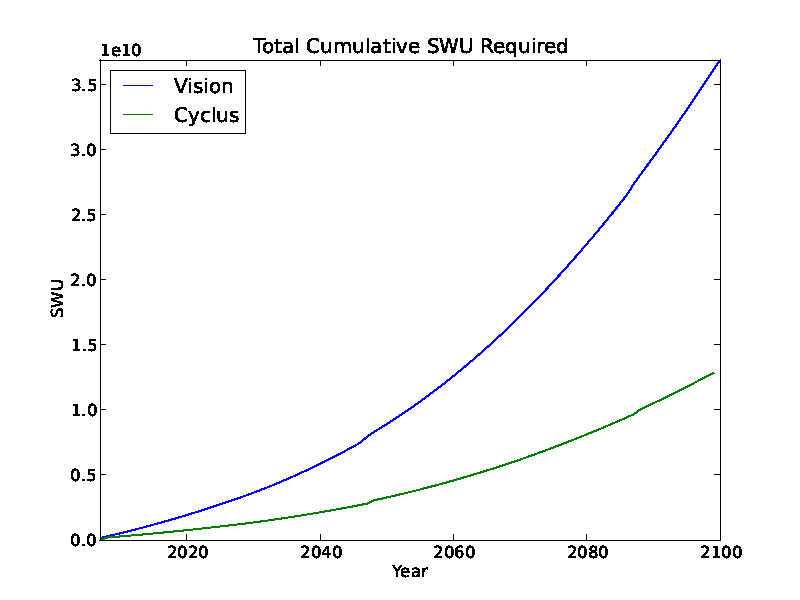
\includegraphics[width=.45\linewidth]{./chapters/prevwork/graphs/swu_low.png}
    \label{fig:swu_low}}
  \quad
  \subfloat[High Case]{%
    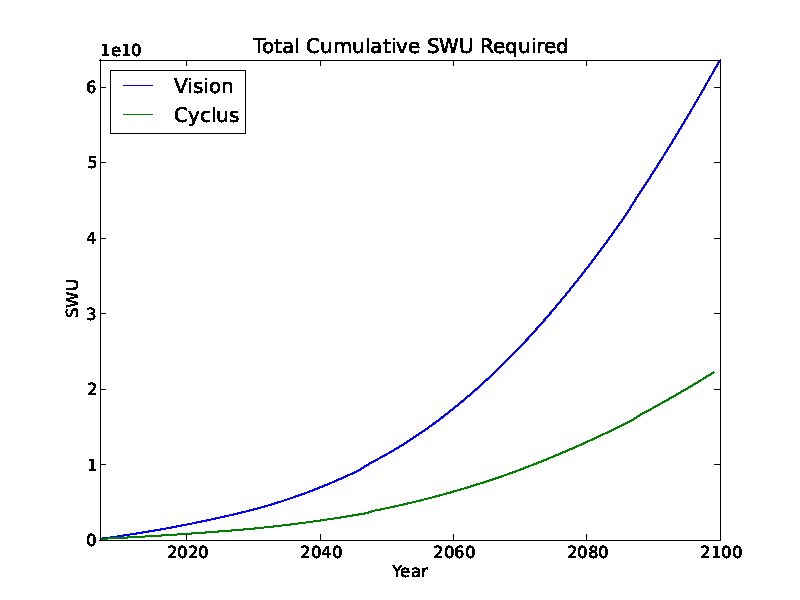
\includegraphics[width=.45\linewidth]{./chapters/prevwork/graphs/swu_high.png}
    \label{fig:swu_high}}
\caption{SWU usage in each INPRO demand case.}
\label{fig:swu}
\end{figure}

\subsection{Benchmark Specification Language}


\chapter{Research Proposal}\label{ch:research}

This chapter seeks to lay out a plan by which a fully agent-based simulation can
be implemented for a generic nuclear fuel cycle with a more realistic chemical
separations and fuel-matching model than currently exists in the field. The term
generic implies that the facilities involved are not known \textit{a priori}
and, accordingly, facilities can be coupled together automatically, separating
the concern of fuel facility modeling and connection from the simulation
solution engine. For example, a modeler has the choice to model a separations
facility and advanced fuel fabrication facility as separate entities whose
connected supply and demand are met by a generic engine, or to model the two
facilities as a single combined and coupled entity. Additionally, the solution
framework for this matching engine must be agnostic as to the classes of
commodities and materials involved. Rather than hard-coding in constraints and
capacities for different material classes, they are added dynamically based on
the entities involved in the simulation-based solution.

As fuel cycle simulators have progressed from simple spreadsheet applications,
work advancing the field has focused on including in-simulation dynamic
calculations of important metrics and parameters in order to provide feedback to
the simulation rather than solely post-processing simulation output. A number of
examples exist. COSI uses the CESAR depletion code \cite{vidal_cesar:_2006} to
automate output fuel characteristics in order to reduce voluminous user input
for simulated materials. Scopatz introduced the notion of essential physics
modeling with his Bright simulation engine \cite{scopatz_essential_2011}. Most
recently, Huff has added to this area of work by developing a repository
facility for the \Cyclus simulator that analyzes repository effects due to
different combinations of materials in different repository
geologies~\cite{huff_integrated_2013}.

This work proposes additional advancement of the dynamic simulation of nuclear
fuel cycles using the \Cyclus simulator. First, a simulation framework for
simulation entity interaction is introduced, the primary goal of which is to
encapsulate simulation-level design decisions. The framework allows for market
interactions to be defined, providing a formalism by which information related
to supply and demand of commodities and materials can be represented in a
general sense. Commodities are not treated simply as quantities, instead the
quantity and \textit{quality} of commodities is treated.  Next, a mathematical
programming formulation based on the multi-commodity transport problem is
proposed to solve the generic supply-demand matching problem. A linear program
formulation and mixed integer-linear program formulation is proposed, the latter
of which addresses the trade-off between computation speed and realism. Finally,
the issue of matching separated elemental streams with requested recycled fuel
is addressed via an approximation linear program.


\section{Agent Interaction in \Cyclus}

\subsection{Facilities}
\subsection{Institutions}
\subsection{Regions}
\subsection{Supply/Demand Resolution Mechanism}

\section{The Generic Fuel Cycle Transportation Problem}

\subsection{Formulation}

In formulating the Generic Fuel Cycle Transportation Problem (GFCTP), note that
the ``players'' in the set of commodity ``markets'' are the individual
facilities involved in the simulation, i.e., the reactors, fabrication
facilities, repositories, etc. In strict mathematical programming parlance, the
GFCTP can be described as a Mixed-Integer, Multicommodity Transportation Problem
(MTP) with Side Constraints. Accordingly are a number of departures from the
classical MTP that was described in \S\ref{sec:MTP}.

To begin, the multicommodity aspect of the problem is not manifest on arc
capacities. Instead, facility demand constraints incorporate a set of
satisfactory commodities. For example, a reactor may be able to accept UOX or
MOX fuel, but has a demand for total fuel. Additionally, supplier facilities may
have a set of constraints on their ability to supply a given commodity and they
may not be able to directly express those constraints with the unit of the
commodity market, i.e., kilograms. Take for example an enrichment facility. Such
a facility has nominally two constraints: SWU capacity and natural uranium
capacity. The former constraint is temporal, i.e., it is a processing
constraint. The latter constraint is an inventory constraint. However, both are
necessary to fully define the problem. Furthermore, let us note that the output
of this facility is kilograms of enriched uranium. Accordingly, the above
capacities must be translated into this output. Finally, realism is introduced
through integer variables. For a number of facilities, especially reactors, it
may not be realistic for a given fuel order to be split amongst a variety of
suppliers. The realm of integer programming techniques allow us to introduced
binary variables to enforce this reality constraint.

It should be noted that the addition of integer variables changes both the
complexity of the formulation and the complexity of the solution technique. Such
a change requires a Mixed Integer-Linear Program (MILP) formulation and solution
via the branch-and-bound method (see \S\ref{sec:bnb}) which solves NP-Hard
combinatorial optimization problems whereas the Linear Program (LP) version
requires the transportation simplex method (see \S\ref{sec:trans-simplex})
which is solvable in polynomial time.  Accordingly, I describe the full
formulation in two parts below: \S\ref{sec:GFCTP-LP} describes the linear
program formulation with side constraints which I will denote GFCTP-LP
and \S\ref{sec:GFCTP-E} describes the MILP formulation with side constraints
which I will denote GFCTP-E (E stands for ``exclusive'', i.e., integer variables
denote an exclusive selection of consumers and/or producers).

\subsubsection{Linear Program with Side Constraints Formulation}\label{sec:GFCTP-LP}


The Generic Fuel Cycle Transportation Problem with Side Constraints (GFCTP-LP)
describes a multi-commodity setting in which demand can be met by multiple
commodities. Consumers denote a cost preference over the possible commodities
they consume and a demand for the set of commodities that must be met. Suppliers
denote one or more production capacities for a given commodity which serve as
the set of supply capacities analogous to the normal MTP
(see \S\ref{sec:MTP}). The GFCTP-LP formulation is as follows:

%%% 
\begin{subequations}\label{eqs:GFCTP-LP}
  \begin{align}
    %%
    \min_{z} \:\: & 
    z = \sum_{h \in H}\sum_{i \in I}\sum_{j \in J}c_{i,j}(h) x_{i,j}(h) 
    & \label{eq:GFCTP-LP_obj} \\
    %%
    \text{s.t.} \:\: &
    \sum_{j \in J}\beta_{i,k}(q_{j}(h)) x_{i,j}(h) \leq s_{i,k} 
    &
    \: \forall \: k \in K_{i}(h),  
    \forall \: i \in I, \forall \: h \in H \label{eq:GFCTP-LP_sup} \\
    %%
    &
    \sum_{i \in I}\sum_{h \in H_{j}} x_{i,j}(h) \geq d_{j}(H_{j}) 
    & 
    \forall \: j \in J \label{eq:GFCTP-LP_dem} \\
    %%
    &
    x_{i,j} \geq 0
    &
    \forall \: x \in X \label{eq:GFCTP-LP_x}
    %%
  \end{align}
\end{subequations}
%%% 

The sets and variables involved are described in Tables \ref{tbl:GFCTP-LP-sets}
and \ref{tbl:GFCTP-LP-vars}.

%%% 
\begin{table} [h!]
\centering
\begin{tabularx}{\textwidth-20pt}{|c|X|} % line wraps second column if too long
\hline
Set         & Description \\
\hline
$H$         & all commodities  \\
$I$         & all producers  \\
$J$         & all consumers  \\
$X$         & the feasible set of flows between producers and consumers  \\
$K_{i}(h)$  & the set of constraining capacities for 
            producer $i$ of commodity $h$  \\
$H_{j}$     & the set of satisfying commodities for consumer $j$  \\
\hline
\end{tabularx}
\caption{Sets Appearing in the GFCTP-LP Formulation}
\label{tbl:GFCTP-LP-sets}
\end{table}
%%% 

%%% 
\begin{table} [h!]
\centering
\begin{tabularx}{\textwidth-20pt}{|c|X|} % line wraps second column if too long
\hline
Variable    & Description \\
\hline
$c_{i,j}(h)$             & the unit cost of commodity $h$ 
                         for producer $i$ and consumer $j$  \\
$x_{i,j}(h)$             & a decision variable, the flow of commodity $h$ 
                         for producer $i$ and consumer $j$  \\
$q_{j}(h)$               & the requested quality of commodity $h$ 
                         by consumer $j$  \\
$\beta_{i,k}(q_{j}(h))$  & a capacity translation function for capacity 
                         constraint $k$ of producer $i$ given $q_{j}(h)$ \\
$s_{i,k}$                & a supply capacity of producer $i$ corresponding to 
                         capacity constraint $k$ \\
$d_{j}(H_{j})$           & the total demand of consumer $j$ over the set of 
                         satisfying commodities $H_{j}$ \\
\hline
\end{tabularx}
\caption{Variables Appearing in the GFCTP-LP Formulation}
\label{tbl:GFCTP-LP-vars}
\end{table}
%%% 

This formulation deviates from the normal MTP formulation via the expansion of
capacity constraints (Equation \ref{eq:GFCTP-LP_sup}) and the inclusion of a
constraint allowing multiple commodities that are able to meet the demand of a
producer (Equation \ref{eq:GFCTP-LP_dem}). The former constraint maintains the
multi-commodity nature of the formulation. This leads to an important insight: if
Equation \ref{eqs:1demand} holds,

\begin{equation}\label{eqs:1demand}
  \left|{H_{j}}\right| = 1 \: \forall \: j \in J
\end{equation}

then the GFCTP-LP can be transformed into a separable multi-commodity
transportation problem as shown in \cite{bertsekas_network_1998}. If the problem
is separable, then the Transportation Problem Simplex Method shown in
\S\ref{sec:trans-simplex} can be applied to a series of smaller subproblems,
reducing overall complexity. Furthermore, if Equations \ref{eqs:1demand} and
\ref{eqs:1constraint} both hold,

\begin{equation}\label{eqs:1constraint}
  \left|{K_{i}(h)}\right| = 1 \: \forall \: i \in I, \: \forall \: h \in H
\end{equation}

then the GFCTP-LP is in fact the a normal Transportation Problem, because the
quality translation function ($\beta_{i,k}(q_{j}(h))$) translates to a constant
at solution time.

\paragraph{Capacity Translation Function and Constraints Example}~\\

The notion of a capacity translation function is something that I have
introduced out of necessity due to the complexity of the GFCTP. Accordingly, an
example will help clarify its purpose. I'll use this time to also to provide an
example of a producer with multiple capacity constraints for a given commodity.

Take, for example, an enrichment facility. Such a facility produces the
commodity ``Enriched Uranium''. This facility has two constraints on its
operation for any given time period: the amount of Separative Work Units (SWU)
that it can process and the total uranium feed it has on hand. Note that neither
of these capacities are measure directly in the units of the commodity it
produces, i.e., kilograms of enriched uranium. We can now state the set the
values for $K_{i}(h)$ for this facility:

\begin{equation}\label{eqs:enr-constr-commods}
  K_{enr}(\mbox{Enriched Uranium}) = \{ \mbox{SWU}, \mbox{Natural Uranium} \}
\end{equation}

Let us now consider that there is a set of requests for enriched uranium that
this facility can possibly meet. Such requests have, in general, two parameters:
$P_{j}$, the total product quantity (in kilograms), and $\varepsilon_{j}$, the
product enrichment (in w/o U-235). Although it would be consistent to use the
notation that has previously been used in \S\ref{sec:prev-enrich}, I will denote
the product weight fraction as $\varepsilon_{j}$ rather than $x_{p,j}$ to reduce
confusion with the similar notation of commodity flow, $x_{i,j}$. In any case,
notice that we have provided the following definition:

\begin{equation}\label{eqs:enr-q-swu}
  q_{j}(\mbox{Enriched Uranium}) \equiv \varepsilon_{j}
\end{equation}

These values are set during a prior phase of the overall matching algorithm, and
can therefore be considered constants. Further, let us note that, in general, an
enrichment facility's operation, or rather its capacity thereof, is governed by
two parameters: $x_{f,enr}$, the fraction of U-235 in its feed material, and
$x_{t,enr}$, the fraction of U-235 in its tails material. Let us assume both of
these are constants of the facility. Utilizing the equations presented in
\S\ref{sec:prev-enrich}, we can denote the functional forms of the arguments of 
this facility's two capacity constraints.

\begin{align}
\label{eqs:enr-prod-beta}
\beta_{enr,NU}(\varepsilon_{j}) = & \:\: \frac{\varepsilon_{j} - x_{t,enr}}
                                      {x_{f,enr} - x_{t,enr}} \\
\begin{split}
\label{eqs:enr-swu-beta}
\beta_{enr,SWU}(\varepsilon_{j}) = & \:\: V(\varepsilon_{j}) \\
                         & + \frac{\varepsilon_{j} - x_{t,enr}}
                                  {x_{f,enr} - x_{t,enr}} V(x_{t,enr}) \\
                         & - \frac{\varepsilon_{j} - x_{f,enr}}
                                  {x_{f,enr} - x_{t,enr}} V(x_{f,enr})
\end{split}
\end{align}

Where $V(x)$ is the value function described in Equation \ref{eqs:enr-value}.
Finally, we can form the set of constraint equations for the enrichment
facility by combining Equations \ref{eq:GFCTP-LP_sup}, \ref{eqs:enr-q-swu}, 
\ref{eqs:enr-prod-beta}, and \ref{eqs:enr-swu-beta}.

\begin{align}
\label{eqs:enr-prod-constr}
\sum_{j \in J}\beta_{enr,NU}(\varepsilon_{j}) \: x_{enr,j}(\mbox{Enriched Uranium})  & \leq s_{enr,NU} \\
\label{eqs:enr-swu-constr}
\sum_{j \in J}\beta_{enr,SWU}(\varepsilon_{j}) \: x_{enr,j}(\mbox{Enriched Uranium}) & \leq s_{enr,SWU}
\end{align}



\subsubsection{Mixed Integer-Linear Program with Side and Exclusivity Constraints Formulation}\label{sec:GFCTP-E}

The previous linear program (LP) formulation of the Generic Fuel Cycle
Transportation Problem fully describes many of the types of transactions that
arise at any given time step. However, it importantly glosses over the critical
case of reactor fuel orders, which comprise a large amount of material orders
within the simulation context. Specifically, it allows reactor fuel orders to be
met by more than one supplier with an arbitrary amount of the order met by each
supplier. Put another way, the LP formulation does not contain the discrete
material information required to model the transaction of fuel assemblies. Such
detail is not necessary in every simulation, but we wish to allow this advanced
modeling for those that do need it. In order to provide this capability of
quantizing orders, binary decision variables must be introduced and integer
programming techniques must be utilized to solve the resulting mixed
integer-linear program. I present the updated formulation below. The key
difference is the inclusion binary variables $y_{i,j}^{h}$, which are 1 if
producer $i$ trades commodity $h$ with consumer $j$ and constants
$\tilde{x}_{j}^{h}$, which denote the quantity of a quantized order. Further a
new set is introduced, $J_{e}$, the set of consumers who require quantized, or
exclusive, orders. The original set of consumers, those who allow partial
orders, I denote $J_{p}$. These two sets constitute the set of all consumers.

\begin{equation}\label{eqs:consumer-union}
  J = J_{p} \cup J_{e}
\end{equation}

The Generic Fuel Cycle Transportation Problem with Exclusive Orders (GFCTP-E)
formulation follows:

\begin{subequations}\label{eqs:GFCTP-E}
  \begin{align}
    %%
    \label{eq:GRCTP-E_obj}
    \min_{z} \:\: 
    & 
    z = \sum_{h \in H}\sum_{i \in I}\sum_{j \in J_{p}}c_{i,j}^{h} x_{i,j}^{h} 
    + \sum_{h \in H}\sum_{i \in I}\sum_{j \in J_{e}}c_{i,j}^{h} y_{i,j}^{h} \tilde{x}_{j}^{h}
    && \\
    %%
    \label{eq:GRCTP-E_sup}
    \text{s.t.} \:\: 
    &
    \sum_{j \in J_{p}}\beta_{i,k}(q_{j}^{h}) x_{i,j}^{h}
    + \sum_{j \in J_{e}}\beta_{i,k}(q_{j}^{h}) y_{i,j}^{h} \tilde{x}_{j}^{h} \leq s_{i,k}^{h} 
    &&
    \forall \: i \in I, \: \forall \: k \in K_{i}^{h}, \forall \: {h \in H} \\
    %%
    \label{eq:GRCTP-E_dem_p}
    &
    \sum_{i \in I}\sum_{h \in H_{j}} x_{i,j}^{h} \geq d_{j}(H_{j}) 
    & 
    \forall \: j \in J_{o} &\\
    %%
    \label{eq:GRCTP-E_dem_e}
    &
    \sum_{i \in I}\sum_{h \in H_{j}} y_{i,j}^{h} \tilde{x}_{j}^{h} \geq d_{j}(H_{j}) 
    &
    \forall \: j \in J_{e}  &\\
    %%
    \label{eq:GRCTP-E_sumy}
    &
    \sum_{h \in H}\sum_{i \in I} y_{i,j}^{h} = 1
    &
    \forall \: j \in J_{e}  &\\
    %%
    \label{eq:GRCTP-E_x}
    &
    x_{i,j}^{h} \geq 0
    &
    \forall \: x \in X  &\\
    %%
    \label{eq:GRCTP-E_y}
    &
    y_{i,j}^{h} \in \{0,1\}
    &
    \forall \: y \in Y &
    %%
  \end{align}
\end{subequations}

The sets and variables involved are described in Tables \ref{tbl:GFCTP-E-sets}
and \ref{tbl:GFCTP-E-vars}. Note that $H_{j}$ is a subset of the commodities:

\begin{equation}
  H_{j} \subseteq H \: \forall \: j \in J_{p}, \forall \: j \in J_{e}
\end{equation}

%%% 
\begin{table} [h!]
\centering
\begin{tabularx}{\textwidth-20pt}{|c|X|} % line wraps second column if too long
\hline
Set         & Description \\
\hline
$H$         & all commodities  \\
$I$         & all producers  \\
$J_{p}$     & all consumers who accept parital orders  \\
$J_{e}$     & all consumers who accept only exclusive orders  \\
$X$         & the feasible set of flows between producers and consumers  \\
$Y$         & the feasible set of exclusive flows between 
            producers and consumers  \\
$K_{i}^{h}$ & the set of constraining capacities for 
            producer $i$ of commodity $h$  \\
$H_{j}$     & the set of satisfying commodities for consumer $j$  \\
\hline
\end{tabularx}
\caption{Sets Appearing in the GFCTP-E Formulation}
\label{tbl:GFCTP-E-sets}
\end{table}
%%% 

%%% 
\begin{table} [h!]
\centering
\begin{tabularx}{\textwidth-20pt}{|c|X|} % line wraps second column if too long
\hline
Variable    & Description \\
\hline
$c_{i,j}^{h}$             & the unit cost of commodity $h$ 
                          for producer $i$ and consumer $j$  \\
$x_{i,j}^{h}$             & a decision variable, the flow of commodity $h$ 
                          for producer $i$ and consumer $j$  \\
$q_{j}^{h}$               & the requested quality of commodity $h$ 
                          by consumer $j$  \\
$y_{i,j}^{h}$             & a binary decision variable that is equal to 1 if 
                          there is flow from producer $i$ to consumer $j$ of 
                          commodity $h$ \\
$\tilde{x}_{j}^{h}$       & the amount of commodity $h$ requested by 
                          consumer $j$ \\
$\beta_{i,k}(q_{j}^{h})$  & a capacity translation function for capacity 
                          constraint $k$ of producer $i$ given $q_{j}^{h}$ \\
$s_{i,k}^{h}$             & a supply capacity of producer $i$ corresponding to 
                          capacity constraint $k$ of commodity $h$ \\
$d_{j}(H_{j})$            & the total demand of consumer $j$ over the set of 
                          satisfying commodities $H_{j}$ \\
\hline
\end{tabularx}
\caption{Variables Appearing in the GFCTP-E Formulation}
\label{tbl:GFCTP-E-vars}
\end{table}
%%%

The examples of the various constraints from the previous section also apply
here. The only difference is the notion of the binary variables, $y_{i,j}^{h}$s,
which denote a sort of on/off switch as to whether a consumer's entire requested
amount of material is met by a supplier or not.

It should be noted that this advanced formulation brings in signifigant
complexity to the resolution method at every time step. As with other mixed
integer-linear programs, the GFCTP-E is NP-Complete and must be solved using the
Branch-and-Bound technique described in \S\ref{sec:bnb}. However, simple
heuristics exist. The most common of them is to solve a relaxed version of the
problem in the form of a linear program, and to round values to form an integer
solution. The exploration of additional heuristics will be performed based on
the outcome of the implementation and analysis of this formulation in
the \Cyclus simulation environment.



\subsection{Cost Function}\label{sec:cost-function}

In any network flow problem, of which transportation problems are a subset, the
cost of transporting commodities is what drives the solution. In other words,
costs are trying to be minimized, and it is the global minimization which
defines an optimal solution. Accordingly, an accurate cost function is
neccessary to determine an accurate solution. Because the \Cyclus simulation
environment is still a nascent technology, accurate pricing metrics, and what
such metrics even are in terms of a centuries-long fuel cycle simulation, are
not immediately available. Accordingly, the cost function is currently a measure
of simulation entity preference, rather than a concrete representation of cost.

The notion of preference extends the work of Kyle Oliver's affininty metric
\cite{oliver_geniusv2:_2009}. The preference metric is generally consumer
centric, i.e., consumers have a preference over the possible commodities that
could meet their demand. For example, a reactor may be able to use UOX or MOX
fuel, but may prefer to use MOX fuel. Herein lies the projection of real-world
cost into the simulation. Additionally, the managers of a given facility, which
in the \Cyclus simulation environment include its Institution and Region, also
exert an influence over its preference. An obvious example is the notion of
affinities given in \cite{oliver_geniusv2:_2009}. In Oliver's work, an affinity
or preference existed between facilities in ``similar'' institutions in order to
drive the trading between institutions as a simple model of international
relations. I expand upon this notion to cover a facility's other managers and
the commodities themselves. Additionally, a preference can be delineated between
the proposed qualities of the same commodity from different vendors. Finally,
the notion of a preference is a positive one, and we require a notion of cost to
solve the minimum-cost formulation of the multicommodity transportation problem
with side constraints. Therefore we must have a translation function.




%\subsection{Benefits and Detriments}

\section{The Recipe Approximation Problem}

The Recipe Approximation Problem (RAP) was originally conceived by Kyle Oliver
in \cite{oliver_geniusv2:_2009}. It was the result of conversations with
scientists of the VISION fuel cycle simulation team \cite{vision2009} with what
was then called the Winery Problem, because of the similarity due to mixing
vintages of win to match a given recipe. This work expands Oliver's initial
formulation by correcting an error and expanding the single-request formulation
to an N-request formulation.

The Recipe Approximation Problem (RAP) seeks to model a separations facility
matching reactor fuel orders. The basic assumptions of the problem are the
following: there are a set of barrels of separated material, $B$, and a set of
fuel requests, $R$, that specify an isotopic vector, $I_{r}$, and quantity,
$q_{r}$, that fully describe a desired fuel order. The goal of the solution
methodology is to determine a matrix of extraction fractions $X$, where each
entry, $x_{b,r}$ denotes the fraction of barrel $b$ being used to match fuel
request $r$. The problem is shown graphically in Figure \ref{fig:rap},
displaying the set of barrels, $B$, the set of fuel requests, $R$, and the set
of extraction fractions, $X$.

\begin{figure}[h]
  \begin{center}
    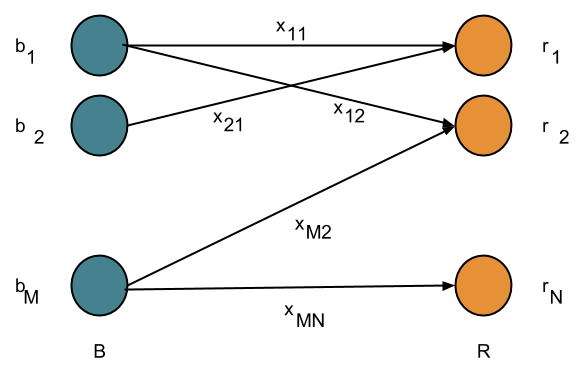
\includegraphics[width=8cm]{./chapters/research/rap.png}
  \caption{A graphical view of an example solution to the Recipe Approximation 
           Problem.}
  \label{fig:rap}
  \end{center}
\end{figure}

The optimal extraction fractions are modeled as the solution to an
approximation linear program, the foundations of which were described in
\S\ref{sec:approx}. Below I describe the most straightforward formulation of 
the RAP, expanding upon the work in \cite{oliver_geniusv2:_2009}. I then
describe how additional constraints can be added to the formulation given
additional information. Finally, I describe a more abstract version that adds a
notion of agency to the problem formulation.



\subsection{Formulation}

The goal of this formuation is to match a set of fuel requests as closely as
possible, where proximity in this sense is defined by the $L^{1}$ norm of the
distance between a mixture attribute and a target attribute. In the following
linear program, the mixture attribute is the dot product of a matrix and a
vector. The matrix is that of all isotopic masses in barrels, $M$, where an
entry, $M_{b,i}$, is the mass of isotope $i$ in barrel $b$. The vector is the
decision variables for a given recipe, $\vec{x_{r}}$, where an entry, $x_{b,r}$,
is the fraction of barrel $b$ being assigned to fuel request $r$. The target
attribute is the target fuel request composition, $\vec{t_{r}}$. where an entry,
$t_{i,r}$, is the mass of isotope $i$ in fuel request $r$.

The minimization objective in and of itself is not necessarily interesting. In
order to enforce physical realities and domain-level knowledge, additional
constraints are added that the result must comply with. These include total
mass, isotopic masses, and neutronics constraints. I present the full
formulation below in Equation \ref{eqs:rap} and explain more fully its
derivation and interpretation in the following paragraphs.

%%% 
\begin{subequations}\label{eqs:rap}
  \begin{align}
    %%
    \min_{z} \:\: & 
    z = \sum_{r \in R} \vec{c_{r}}^{\top} \cdot \vec{y_{r}}
    & \label{eqs:rap_obj} \\
    %%
    \text{s.t.} \:\: &
    \vec{y_{r}} = \left| M \cdot \vec{x_{r}}  - \vec{t_{r}} \right|
    &
    \: \forall \: r \in R \label{eqs:rap_iso} \\
    %%
    &
    \epsilon_{m} \geq \left| \sum_{b \in B} m_{b} x_{b,r} - m_{r} \right|
    & 
    \forall \: r \in R \label{eqs:rap_mass} \\
    %%
    &
    \epsilon_{\eta} \sum_{b \in B} \eta_{b}^{-} x_{b,r} \geq 
    \left| \sum_{b \in B} \eta_{b}^{+} x_{b,r} - 
           \eta_{r} \sum_{b \in B} \eta_{b}^{-} x_{b,r} \right|
    & 
    \forall \: r \in R \label{eqs:rap_eta} \\
    &
    \sum_{r \in R} x_{b,r} \leq 1
    & 
    \forall \: b \in B \label{eqs:rap_conserv} \\
    &
    x_{b,r} \in \left[ 0, 1 \right]
    & 
    \forall \: b \in B, \forall \: r \in R  \label{eqs:rap_x}
    %%
  \end{align}
\end{subequations}
%%% 

Let me begin the discussion of the RAP formulation by noting that the
$\vec{y_{r}}$ variables occur twice, once as an assignment in
Equation \ref{eqs:rap_iso} and again in Equation \ref{eqs:rap_obj}, the
objective function. The $\vec{y_{r}}$ variables are column vectors that
represent the different between the isotopic composition of a proposed mixed
solution for a target fuel request, $r$, and the target fuel request itself. The
goal of this formulation is to minimize that difference. However, a strict
difference minimization is not directly suitable. Because separations plants can
separate materials only on elemental scales, not on isotopic scales, and because
fuel recipes are isotopic-specific, there will inevitively be isotopes present
in the barrels that are not requested in the recipe. This is described formally
in Equation \ref{eqs:barrel-req-iso}.

\begin{equation}
\label{eqs:barrel-req-iso}
I_{B} \supseteq I_{r} \: \forall r \in R
\end{equation}

Additionally, the isotopes that are most important from a nuclear engineering
domain knowledge point of view are known to of relatively low concentration in
the final fuel recipe (e.g., U-235 is only 3-5 w/o of LWR fuel). Accordingly,
some kind of weighting function is required to determine the relative importance
among isotopes in the resulting solution. I adopt Oliver's definition of this
weight from \cite{oliver_geniusv2:_2009}, which normalizes the importance of
isotopes in the final mixture.

\begin{equation}
c_{i,r} = 
\begin{cases}
 \frac{1}{m_{i,r}} & \text{if } i \in I_{r} \\
 \frac{1}{m_{r}}   & \text{if } i \not\in I_{r}
\end{cases}
\end{equation}

Note that the dot product of the vectors $\vec{y_{r}}$ and $\vec{c_{r}}^{\top}$
results in a scalar, and we wish to minimize the aggregate sum of scalars for
all fuel requests.

Moving on to the physical constraints, let us cover the simpler
Equation \ref{eqs:rap_mass} first. This constraint states that the mass of a
feasible matching solution, i.e. $\sum_{b \in B} m_{b} x_{b,r}$, must be within
some range of the mass of the given fuel request, $m_{r}$. This range is defined
by some small value, $\epsilon_{m}$. It is important to realize that the
$\epsilon$ vaules appearing in these constraints critically affect the
feasibility space. Whereas the objective function seeks to minimize the
difference between a mixture attribute and target attribute, the $\epsilon$
values define a maximum allowable difference. Accordingly, the define the bounds
of the feasible solution space. It entirely possible that during the course of a
simulation, an instance of the RAP will not have a feasible solution. In such a
scenario, the various $\epsilon$ values will have to be incrementally increased,
or relaxed, until feasibility is attained.

The neutronics constraint, Equation \ref{eqs:rap_eta}, is more complicated and
deserves its own derivation. First, note its purpose. It is a constraint on the
neutronics parameter $\eta$, i.e., the number of neutrons produced per fission
per absorption in the fuel. It is a material-specific value, which is to say
that it is a function only of material properties of the fuel, rather than the
reactor geometry or the material properties of the fuel or the moderator, as are
most other neutronics-related parameters, e.g., the effective multiplication
factor, $k_{eff}$. This parameter is ideal for an initial attempt at this
formulation because it requires only the minimal information associated with
material requests in \Cyclus, i.e., a quantity and an isotopic profile. The
equation for $\eta$ of a homogenous medium is as follows.

\begin{equation}
\label{eqs:eta_macro}
\eta = \frac{\sum_{i \in I} \nu^{i} \Sigma_{f}^{i}}
            {\sum_{i \in I} \Sigma_{a}^{i}}
\end{equation}

In Equation \ref{eqs:eta_macro}, $I$ is the set of isotopes in the material,
$\nu^{i}$ is the average neutrons produced per fisison of isotope $i$,
$\Sigma_{f}^{i}$ is the macroscopic cross section for fission of isotope $i$,
and $\Sigma_{a}^{i}$ is the macroscopic cross section for absorption of isotope
$i$. The ratio of the two cross sections produces the probability that a neutron
causes fission given that is absorbed by isotope $i$. For our purposes, because
we do not know how much of each material will contribute to a final mixture, it
is more ideal to work with microscopic cross sections and number densities of an
isotope $i$, $N^{i}$, as shown in Equation \ref{eqs:eta_micro}.

\begin{equation}
\label{eqs:eta_micro}
\eta = \frac{\sum_{i \in I} \nu^{i} \sigma_{f}^{i} N^{i}}
            {\sum_{i \in I} \sigma_{a}^{i} N^{i}}
\end{equation}

In order to discuss this in terms of barrel fractions, we must include them as
multiples of the number densities. 

\begin{equation}
\label{eqs:eta_fractions_nonlin}
\eta_{B} = \frac{\sum_{i \in I_{B}} \nu^{i} \sigma_{f}^{i} \sum_{b \in B} N_{b}^{i} x_{b}}
                {\sum_{i \in I_{B}} \sigma_{a}^{i} \sum_{b \in B} N_{b}^{i} x_{b}}
\end{equation}

In Equation \ref{eqs:eta_fractions_nonlin}, $I_{B}$ denotes the set of all
isotopes in barrels, $N_{b}^{i}$ denotes the number density of isotope $i$ in
barrel $b$, and $\eta_{B}$ is the reproduction factor resulting from the
specific values of barrel fractions $x_{b}$. If we were to leave the definition
of $\eta_{B}$ in this form, we could formulate the constraint in
Equation \ref{eqs:rap_eta} in the same way as is done in
Equation \ref{eqs:rap_mass}.

\begin{equation}
\label{eqs:eta_nonlin}
\epsilon_{\eta} \geq \left| 
\frac{\sum_{i \in I_{B}} \nu^{i} \sigma_{f}^{i} \sum_{b \in B} N_{b}^{i} x_{b,r}}
     {\sum_{i \in I_{B}} \sigma_{a}^{i} \sum_{b \in B} N_{b}^{i} x_{b,r}} 
- \eta_{r} \right|
\: \forall \: r \in R
\end{equation}

$\eta_{r}$ in Equation \ref{eqs:eta_nonlin} is defined in the normal way.

\begin{equation}
\label{eqs:eta_r}
\eta_{r} = \frac{\sum_{i \in I_{r}} \nu^{i} \Sigma_{f}^{i}}
                {\sum_{i \in I_{r}} \Sigma_{a}^{i}}
\end{equation}

Furthermore, $\eta_{r}$ is presumed to be predefined and is a constant with
respect to the RAP. Equation \ref{eqs:eta_nonlin} presents a problem; it
introduces a ratio of decision variables, which is a nonlinearity. In general,
nonlinear programs are much more difficult to solve than linear programs and
require much more exotic techniques. Some algebra can relieve this issue,
however. We begin by massaging Equation \ref{eqs:eta_nonlin}, reformulating it
into Equation \ref{eqs:eta_fractions_nonlin}.

\begin{equation}
\label{eqs:eta_fractions_lin}
\eta_{B} = \frac{\sum_{b \in B} x_{b} \sum_{i \in I_{b}} \nu^{i} \sigma_{f}^{i} N_{b}^{i}}
                {\sum_{b \in B} x_{b} \sum_{i \in I_{b}} \sigma_{a}^{i} N_{b}^{i}}
\end{equation}

Note that out of Equation \ref{eqs:eta_fractions_nonlin} fall two parameters
that are defined for each barrel, which I denote $\eta_{b}^{+}$ and
$\eta_{b}^{-}$.

\begin{equation}
\label{eqs:eta_+}
\eta_{b}^{+} \equiv \sum_{i \in I_{b}} \nu^{i} \sigma_{f}^{i} N_{b}^{i}
\end{equation}

\begin{equation}
\label{eqs:eta_-}
\eta_{b}^{-} \equiv \sum_{i \in I_{b}} \sigma_{a}^{i} N_{b}^{i}
\end{equation}

Equations \ref{eqs:eta_+} and \ref{eqs:eta_-} allow us to write
Equation \ref{eqs:eta_fractions_lin} more simply.

\begin{equation}
\label{eqs:eta_simple}
\eta_{B} = \frac{\sum_{b \in B} \eta_{b}^{+} x_{b}}
                {\sum_{b \in B} \eta_{b}^{-} x_{b}}
\end{equation}

We can then rewrite Equation \ref{eqs:eta_nonlin} using
Equation \ref{eqs:eta_simple}.

\begin{equation}
\label{eqs:eta_nonlin_simple}
\epsilon_{\eta} \geq \left| 
\frac{\sum_{b \in B} \eta_{b}^{+} x_{b_r}}
     {\sum_{b \in B} \eta_{b}^{-} x_{b_r}}
- \eta_{r} \right|
\: \forall \: r \in R
\end{equation}

Finally, we can multiply Equation \ref{eqs:eta_nonlin_simple} through by the
denominator of Equation \ref{eqs:eta_simple} to arrive at the form of the
constraint in \ref{eqs:rap_eta}.

\begin{equation}
\label{eqs:eta_linear}
\epsilon_{\eta} \sum_{b \in B} \eta_{b}^{-} x_{b,r} \geq
\left| \sum_{b \in B} \eta_{b}^{+} x_{b,r}
- \eta_{r} \sum_{b \in B} \eta_{b}^{-} x_{b,r} \right|
\: \forall \: r \in R
\end{equation}

The constraint in Equation \ref{eqs:eta_linear} has been linearized, and the
polynomial-time Simplex Method can again be applied as the solution mechanism. 

Finally, let me discuss Equations \ref{eqs:rap_conserv} and \ref{eqs:rap_x}.
Equation \ref{eqs:rap_conserv} simply states that the sum of all barrel
fractions for any given barrel must be less than one. This is simply a check on
reality -- you can't take more things from a container than exist in the
container in the first place. Equation \ref{eqs:rap_x} simply defines the notion of
a fraction, saying that all barrel fractions must lie in the range of 0 and 1,
inclusive.


\subsubsection{Additional Constraints}
\subsubsection{Agency and Abstraction}
\subsection{Initial Results and Benchmarks}


%% etc, etc.

%% Do you have appendices?  If so, add them here, just like chapters.
% \begin{appendices}
% \chapter{\Cyclus To Date}\label{sec:cyclus}

Significant, strategic improvements have been added to the \Cyclus code base.
Interactions with dynamically-loadable libraries and reading XML-input files
have been encapsulated in classes and enhanced. 

\section{Dynamic Loading}\label{sec:prev-dynamic}

Software libraries can be accessed in a static manner, i.e., they are connected
to an application during the linking phase of building a program, or can be
accessed in a dynamic manner, i.e., they are connected at run time. Dynamic
linkage, or dynamic loading, is a well-known technique for to support
connectable, modular components, or plug-ins. \Cyclus utilizes a plug-in
approach for its facility, institution, and region agent libraries. This design
decision furthers the \Cyclus development goal of providing an agnostic
framework into which sophisticated users can develop different models of agents
to investigate specific simulation-modeling change.

Work was performed in order to use class-based representation of dynamic
libraries, allowing for easy opening, closing, and access thereof. Each dynamic
library represents an agent type in \Cyclus, providing a constructor and
destructor. The DynamicModule class then provides the \Cyclus core access to
these constructors and destructors to perform the appropriate operations at run
time. Because dynamic loading is treated differently on POSIX-based systems than
it is on Windows-based systems, specialty functions for library access were
provided for each system. The correct header file (UnixHelperFunctions.h or
WindowsHelperFunctions.h) is chosen during compilation. 

These changes simplified the client code that utilizes library access. The
\Cyclus core application can now call appropriate library-related functions in
an agnostic manner. Specific, well-defined time points of module loading
(dynamic library opening) and unloading (dynamic library closing) were defined
in the \Cyclus application. These operations, called by the application,
currently reside in the Model class and could likely be refactored into a
specific handler class designed for this purpose.

\section{Input Reading}

A large overhaul to the input-reading code base was performed. \Cyclus currently
only supports XML input files that adhere to the RNG schema defined in the
\Cyclus RNG file. However, it is a well-known best practice to provide an
agnostic application programming interface (API) that can be configured with
specific class instances given some user-defined input. Accordingly, such an API
was constructed which currently supports XML input but can also support future
input types that are tree-based (e.g., JSON, CSV, etc.).

The top-level abstraction is encased in a QueryEngine class. Basic operations
are provided assuming a tree-based input formation, including querying the
number of child elements at the current reading level, the name of each element,
and access to each element. The application code is responsible for configuring
the appropriate input parser and populating an instance of a QueryEngine at its
root. The client code then populates input parameters through the QueryEngine
interface rather than an input-format specific interface.

Support for XML-file reading has been enhanced by separating various concerns
into appropriate classes. Four classes have been constructed with specific
purposes regarding input file reading: file loading (XMLFileLoader), file
validation (RelaxNGValidator), file parsing (XMLParser), and querying
(XMLQueryEngine). The application interfaces with the file loader, initializing
it with a given input file path and then invoking the loading of various
\Cyclus-specific parameters (e.g., simulation control parameters, material
recipes, agent modules, etc.). The loader is responsible for managing its parser
and providing client code with correctly-configured instances of
XMLQueryEngines. The parser is responsible for providing an interface to the
underlying C++ XML parsing library (i.e., libxml++) and invoking the appropriate
validation routines on the parsed file. The validator is responsible for
providing access to the RNG-validation operations through libxml and
libxml++. Finally, the XML-specific derived QueryEngine class is responsible for
implementing XML querying using the generic QueryEngine interface.

Other input file formats can be supported by providing the appropriate
format-specific derived QueryEngine class and adjusting the application code as
necessary. A developer could then choose how to implement the loading and
validation, if any, of the input file. The structure described above is just one
of many ways to achieve such a goal.

% \end{appendices}

%% Are you a big nerd with a colophon?  Add it here.
% \begin{colophon}
% %\svnidlong{$LastChangedBy$}{$LastChangedRevision$}{$LastChangedDate$}{$HeadURL: http://freevariable.com/dissertation/trunk/frontmatter.tex $}
%\vcinfo{}

This template uses Gyre Pagella by default.  (I used Arno Pro in my dissertation.)

Feel free to give me a shout-out in your colophon or acks if this template is useful for you.  Good luck!

% \end{colophon}

%% McBride is a very nice style (some version is included in this distribution)
\bibliographystyle{mcbride}
\bibliography{refs}

%% Want an index?  Neither did I.
%\printindex

\end{document}
